\documentclass[a4paper]{report}
\usepackage[english]{babel}
\usepackage{amssymb}
\usepackage{amsmath}
\usepackage{graphicx}
\usepackage{float}
\usepackage{shortvrb}
\usepackage{cancel}
\usepackage[T1]{fontenc}
\usepackage{nicefrac}
\usepackage{amsfonts}
%nomenclature
\usepackage{makeidx}
\makeindex
\usepackage{nomencl}
\makenomenclature
\renewcommand{\nomname}{List of Symbols}

\usepackage{standalone} %Makes it possible to ignore other preambles of child document
\usepackage{eurosym} %Euro teken mogelijk
\usepackage{multirow} %For multiple rows togheter in one table
\usepackage{parskip} %For a small white line between paragraphs
\usepackage[protrusion=true,expansion=true]{microtype}
\usepackage{hyperref}%For automatic and URL Reference
\usepackage[titletoc]{appendix}
%Possible to change the margins
\usepackage{geometry}
\geometry{verbose,tmargin=1.9cm,bmargin=1.7cm,lmargin=1cm,rmargin=1cm}

\usepackage{subfig}

%include pdf pages
\usepackage{pdfpages}

%Small titles
\usepackage[small,compact]{titlesec}

%being able to create tables over multiple pages
\usepackage{longtable}

\makeatletter

%Change standard font size
\renewcommand\normalsize{ \@setfontsize\normalsize{11pt}{11pt}}\normalsize  
\makeatother

\usepackage{fancyhdr}
\pagestyle{fancy}
\fancyhead{}
\fancyfoot{}

%Gives text above each page
\fancyhead[CO,CE]{DSE Project}

%Page number
\fancyfoot[RO,LE]{\thepage}


\usepackage{babel}

\newcommand*{\titleDSE}{\begingroup% Three Men in a Boat
\newlength{\drop}
\setlength{\drop}{0.1\textheight}
\centering
\begin{figure}[h!]
\centering

\includegraphics[scale=0.5]{Figures/TUdelftLogo.jpg}
\end{figure}
\settowidth{\unitlength}{\LARGE AAAAAAAAAAAAAAAAAAAAAAAAAAAAAAAAAAAAAA}

\rule{\unitlength}{1.6pt}\vspace*{-\baselineskip}\vspace*{2pt}
\rule{\unitlength}{0.4pt}\\[\baselineskip]
{\LARGE Project Plan}\\[\baselineskip]			%Main Title
{\itshape DSE All Plastic UAV}\\[0.2\baselineskip]					%subtitle
\rule{\unitlength}{0.4pt}\vspace*{-\baselineskip}\vspace{3.2pt}
\rule{\unitlength}{1.6pt}\\[\baselineskip]
\vspace*{0.1\drop}

\begin{figure}[h]
\centering
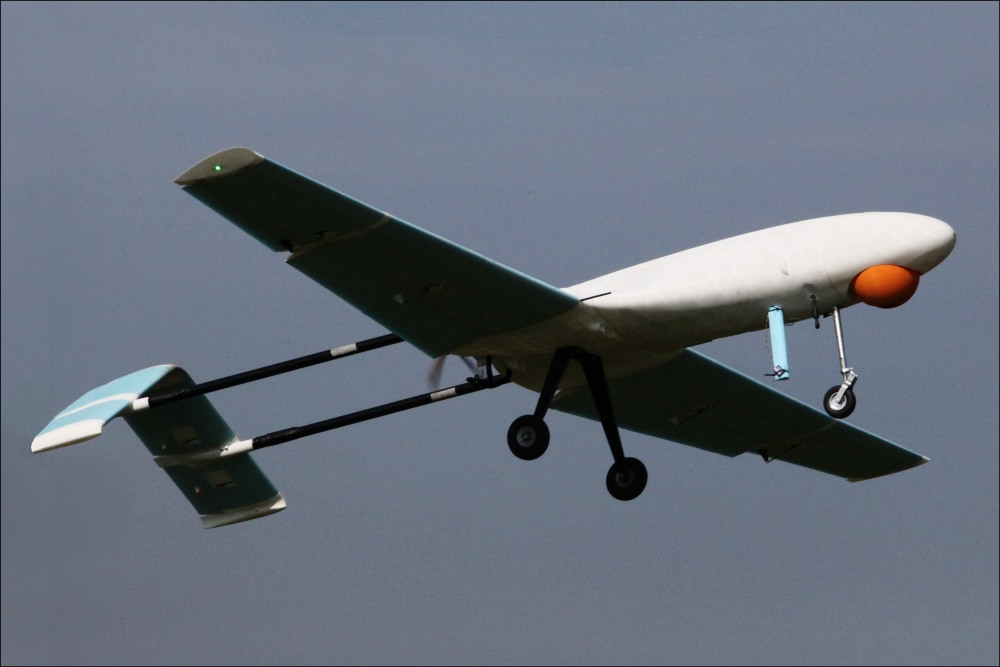
\includegraphics[width =0.75 \textwidth]{Figures/TitleImage.jpg}
\end{figure}
\vfill

\begin{table}[h]
\subfloat{
\begin{tabular}{l l}
\multicolumn{2}{l}{\textbf{Tutors}} \\
\\
Prof. dr. ir. Dingemans, T. & TU Delft\\
Ir. Melkert J. & TU Delft\\
\\
\multicolumn{2}{l}{\textbf{Coaches}}\\
\\
Ir. Bos, R. & TU Delft\\
Ir. Udluft H. & TU Delft
\end{tabular}
}
\hfill
\subfloat{
\begin{tabular}{r r}
\multicolumn{2}{r} {\textbf{Group members}} \\
\\
d. Heij, B. & 1507095 \\
Jeliazkov, M.K. & 4105826 \\
Kerssemakers, M.A.P. & 4005880\\
V.D. Kieboom, B. & 4114752 \\
Mooi, K. & 4020367 \\
Roelofs, M.N. & 4077407 \\
Seelen, J. & 1317547\\
v. Stralen, R. & 4019342 \\
Vendrig, P.R. & 4023838 \\
Verhoeff, C.K. & 1114344 \\
\end{tabular}
}
\end{table}

\endgroup}

%Available structures:
%Report: \part{}, \chapter{}, \section{}, \subsection{}, \subsubsection{}, \paragraph{}, \subparagraph{}

\begin{document}

\begin{titlepage}
\titleDSE
\end{titlepage}
\setcounter{page}{1} %numbering starts from here
\tableofcontents
\newpage
\printnomenclature

\documentclass[a4paper]{report}
\usepackage[english]{babel}
\usepackage{amssymb}
\usepackage{amsmath}
\usepackage{graphicx}
\usepackage{float}
\usepackage{shortvrb}
\usepackage{cancel}
\usepackage[T1]{fontenc}
\usepackage{nicefrac}
\usepackage{amsfonts}

%nomenclature
\usepackage{makeidx}
\makeindex
\usepackage{nomencl}
\nomlabelwidth=20mm
\makenomenclature
\renewcommand{\nomname}{List of abbreviations}

\usepackage{standalone} %Makes it possible to ignore other preambles of child document
\usepackage{eurosym} %Euro teken mogelijk
\usepackage{multirow} %For multiple rows togheter in one table
\usepackage{parskip} %For a small white line between paragraphs
\usepackage[protrusion=true,expansion=true]{microtype}
\usepackage{hyperref}%For automatic and URL Reference
\usepackage[titletoc]{appendix}
%Possible to change the margins
\usepackage{geometry}
\geometry{verbose,tmargin=1.9cm,bmargin=1.7cm,lmargin=1cm,rmargin=1cm}

\usepackage{subfig}

%include pdf pages
\usepackage{pdfpages}

%being able to create tables over multiple pages
\usepackage{longtable}

\makeatletter

%Change standard font size
\renewcommand\normalsize{ \@setfontsize\normalsize{11pt}{11pt}}\normalsize  
\makeatother

\usepackage{fancyhdr}
\pagestyle{fancy}
\fancyhead{}
\fancyfoot{}

%Gives text above each page
\fancyhead[CO,CE]{DSE Project}

%Page number
\fancyfoot[RO,LE]{\thepage}


\usepackage{babel}

%Available structures:
%Report: \part{}, \chapter{}, \section{}, \subsection{}, \subsubsection{}, \paragraph{}, \subparagraph{}

\begin{document}
\chapter{Introduction (1 page)}\label{chap:Intro}
This is the Baseline Review
\end{document}
\documentclass[a4paper]{report}
\usepackage[english]{babel}
\usepackage{amssymb}
\usepackage{amsmath}
\usepackage{graphicx}
\usepackage{float}
\usepackage{shortvrb}
\usepackage{cancel}
\usepackage[T1]{fontenc}
\usepackage{nicefrac}
\usepackage{amsfonts}
\usepackage{standalone} %Makes it possible to ignore other preambles of child document
\usepackage{eurosym} %Euro teken mogelijk
\usepackage{multirow} %For multiple rows togheter in one table
\usepackage{parskip} %For a small white line between paragraphs
\usepackage[protrusion=true,expansion=true]{microtype}
\usepackage{hyperref}%For automatic and URL Reference
\usepackage{appendix}
%Possible to change the margins
\usepackage{geometry}
\geometry{verbose,tmargin=1.9cm,bmargin=1.8cm,lmargin=2cm,rmargin=2cm}

\usepackage{subfig}

%include pdf pages
\usepackage{pdfpages}

%being able to create tables over multiple pages
\usepackage{longtable}

\makeatletter

%Change standard font size
\renewcommand\normalsize{ \@setfontsize\normalsize{11pt}{11pt}}\normalsize  
\makeatother

\usepackage{fancyhdr}
\pagestyle{fancy}
\fancyhead{}
\fancyfoot{}

%Gives text above each page
\fancyhead[CO,CE]{DSE Project}

%Page number
\fancyfoot[RO,LE]{\thepage}


\usepackage{babel}

%Available structures:
%Report: \part{}, \chapter{}, \section{}, \subsection{}, \subsubsection{}, \paragraph{}, \subparagraph{}

\begin{document}
\chapter{Project Definition}
To get a clear understanding of the project and to be able to finish it successfully the Project Objective (PO) and Mission Need Statement (MNS) need to be defined. These statements will be referred to during the entire project to assess the validity of the outcome. Both the PO and MNS can be deduced from a problem statement.

This chapter consists of five sections. ~\autoref{sec:ProblemStatement} gives a description of the problem / context of the project. From this description, the PO is deduced in ~\autoref{sec:ProjectObjective} and the MNS in ~\autoref{sec:MissionNeedStatement}. Next, the top level requirements are presented in ~\autoref{sec:TopLevelRequirements}, followed by a system description in ~\autoref{sec:SystemDescription}.

\section{Problem Statement}
\label{sec:ProblemStatement}
The aerospace industry is increasingly using lightweight polymer-reinforced composites as structural components. This results in fast and fuel-efficient aircraft, like the Boeing 787 'Dreamliner'. Simultaneous to this development, polymers have emerged to be used as flexible, light-weight electronics. Now, they can be used as LEDs, solar cells, transistors, batteries and actuators.

Polymers seem to be very interesting materials, also in the aerospace industry. However, introducing a new material in passenger airplanes can take 10 to 15 years. It would be convenient to reduce this time and be able to follow the rapid developments. A solution is to use UAVs as test bed for these new materials.

A specific UAV to be designed is an observation platform which must remain at a given location for one full year to perform observations. It should not be bothered by air traffic, so the cruise altitude is at least 15 km. For station keeping, wind speeds at these altitudes should be taken into account.

By designing this UAV several questions can be answered: Is it possible to develop such a system from plastics alone? What changes the use of polymers in design, since they can be multi-functional? What will such a system look like and how will it operate? What are the advantages and limitations of such an approach?

\section{Project Objective}
\label{sec:ProjectObjective}
From the problem statement it becomes clear that a UAV should be designed to demonstrate the use of multi-functional plastics. Therefore, the Project Objective can be stated as follows:\\
{\textit "Design a fully multi-functional plastics, high altitude observation platform for a mission of one year at moderate latitudes by 10 students in 11 weeks."}

Because this project is performed for educational purposes within a limited time the aim is not to produce a industrial-worthy, flawless end-result. Although it is very important to iterate design choices for design experience, this process has a limited time-frame and does not have to produce the optimal outcome.

Equally important is the execution of the project, which comprises elements like performing an integrated project and operating as a team. Communication with tutors, coaches and other members of the faculty is also a valuable aspect.
\section{Mission Need Statement}
\label{sec:MissionNeedStatement}
To identify what the product to be designed has to comprise, the Mission Need Statement is deduced from the problem statement. It will provide a check whether the design objective set by the customer(s) is correctly understood and will form a basis for the requirements discovery tree. The Mission Need Statement defined for this product is as follows:\\
{\textit "Observe the Earth with sufficient accuracy to spot individuals from a stationary position above all air traffic for one year."}
\section{Top Level Requirements}
\label{sec:TopLevelRequirements}
For the system, some top level requirements are given. From these requirements, some more specific requirements will be derived, but these will be treated in the following report. Apart from the given list, important requirements are the use of multifunctional parts and that most of the aircraft will consist of "plastic" materials.\\
The following list shows the top level requirements given to us.
\begin{itemize}
\item Maximum take-off mass is not limited
\item The size of the aircraft is not limited, but needs to be practical in operation (ground operation e.g.)
\item Take-off and landing must be possible in wind force 3 conditions
\item Maximum cross wind during take-off and landing of 5 kts
\item Cruise altitude above all traffic, 15 km or above
\item Cruise will take place between 0$^\circ$ and 55$^\circ$ latitude
\item At cruise altitude, a 90\% station keeping must be guaranteed
\item Able to fly non-stop for one full year
\item Payload mass is limited to a maximum of 3 kg
\item Payload should be kept at operating temperature with minimum power usage, preferably below 25 W
\item The payload should be able to track individuals on the ground from cruise altitude, night vision is a plus
\item On board energy storage is allowed
\item Communication and data handling must be designed
\item The costs of a mission should be less than 1 million euro based on a series of 100 devices.
\item Sustainability will be taken into account
\item Stealth characteristics shall be included
\end{itemize}
These requirements must be met by the design. They are the base for further specification on system requirements. Some system requirements will be about the resolution, the frame rate, link-budget and power needed. These will be specified more in the Baseline report. The top level requirements can be used to give a description about the entire system in very general terms.
\section{Description of Entire System}
\label{sec:SystemDescription}
From the requirements it is clear that the system is about observation from a stationary platform at high altitude. This mission will need different subsystems that will be described now.

First of all, the aircraft will have to take-off. A ground crew will be needed to assist with this. This ground crew will also give information to the UAV on target area and objectives. After take-off, it will fly autonomously to the cruise altitude and after that to the target area. Therefore it will need a system to determine it's location and flight path. Also, a propulsion system is needed to be able to cruise. When it reaches the target area, it must be able to remain stationary and observe the ground. Since it needs to be able to track movements of individuals on the ground, some sort of camera needs to be on board with sufficient resolution and field of view. 

Because this data is needed in real time, and not after the end of the mission one year later, communication with the ground is needed. This is necessary in two ways, because commands can be send to the UAV as well. The link budget is important for the amount of data that can be produced by the payload. Again, a ground crew is needed for processing the data. After mission completion, the UAV needs to be able to fly back to base and land safely. It will preferably be reusable for a new mission.

The UAV itself will need to stay in the air non-stop for one full year. Because all of the above requires energy, an important system will be the energy system. Whether all the energy is stored pre-flight or energy will be regained during flight, it will play an important role in the design.
\end{document}
\documentclass[a4paper]{report}
\usepackage[english]{babel}
\usepackage{amssymb}
\usepackage{amsmath}
\usepackage{graphicx}
\usepackage{float}
\usepackage{shortvrb}
\usepackage{cancel}
\usepackage[T1]{fontenc}
\usepackage{hyperref}
%Makes it possible to ignore other preambles of child document
\usepackage{standalone}

%Possible to change the margins
\usepackage{geometry}
\geometry{verbose,tmargin=1.9cm,bmargin=1.8cm,lmargin=2cm,rmargin=2cm}

\usepackage{subfig}

%include pdf pages
\usepackage{pdfpages}

%being able to create tables over multiple pages
\usepackage{longtable}

\makeatletter

%Change standard font size
\renewcommand\normalsize{ \@setfontsize\normalsize{11pt}{11pt}}\normalsize  

\makeatother

\usepackage{fancyhdr}
\pagestyle{fancy}
\fancyhead{}
\fancyfoot{}

%Gives text above each page
\fancyhead[CO,CE]{DSE Project}

%Page number
\fancyfoot[RO,LE]{\thepage}

\usepackage{babel}

%Available structures:
%Report: \part{}, \chapter{}, \section{}, \subsection{}, \subsubsection{}, \paragraph{}, \subparagraph{}

\begin{document}
\chapter{Team organization}
\label{Chapter:Teamorganization}
In this chapter the team organization is presented and elaborated upon. First the individual skills of each team member within a team are investigated, after which the tasks are divided. Next, specialist teams were formed for different disciplines. The visualisation of the final organization is shown by means of an organogram. \\

The team started organising itself by investigating the personalities of the team members, to see what type of role each team member could be assigned to. This was done by using a Belbin\cite{website:belbin} self-perception test, which indicates a percentage score for different types of characters. The results of this test are shown in  \autoref{tab:belbin}. The required positions within the team were determined as well, in order to have responsibility for every aspect of the project work including the software used. The following roles were defined:

\begin{itemize}
\item Chairman
\item Secretary
\item Quality Assurance (2 positions)
\item Systems Engineering (2 positions)
\item MATLAB coordinator
\item CATIA coordinator
\item LATEX coordinator
\item Presentation \& Poster coordinator

\end{itemize}


\begin{table}[h]
\centering
\caption{Main 'Belbin' team roles}
\label{tab:belbin}
   \begin{tabular}{| l | c | } \hline
   
     \textbf{Team member} & \textbf{Main role(s)}  \\ \hline
     Momchil Jeliazkov & Specialist  \\ \hline
     Ties Kerssemakers & Implementer  \\ \hline
     Kevin Mooi & Implementer, Teamworker  \\ \hline
     Martjn Roelofs & Shaper  \\ \hline
     Jannick Seelen & Shaper  \\ \hline
     Bas Van den Kieboom & Teamworker, Implementer  \\ \hline
     Perrin Vendrig & Monitor Evaluator, Implementer  \\ \hline
     Carel Verhoeff & Monitor Evaluator  \\ \hline
     Boudewijn de Heij & Implementer  \\ \hline
     Rick van Stralen & Monitor Evaluator \\ \hline
    
     \end{tabular}
\end{table}

The chairman will take the responsibility of checking all team members to do their assigned tasks and work effectively, as well as keeping track of the progress of the project by means of checklists such that deadlines and deliverables are met at specified times. The secretary keeps track of all decisions made during group discussions and notes issues and questions regarding the project. The Quality Assurance team makes sure that all documents and deliverables are of sufficient quality, both technically as well as visually. The System Engineering team keeps track of the communications and the flow of information between different groups such that all team members get the correct inputs when needed and deliver the right outputs to the right groups on time. The MATLAB coordinator is responsible for the MATLAB part of the project and makes sure that issues with this program can be solved. The CATIA coordinator is responsible for the CATIA deliverables and makes sure these have sufficient quality. The LATEX coordinator is in charge of the LATEX files and the structure of the documents. The Presentation \& Poster coordinator makes sure that the presentations and poster are made before the respective deadlines and have the correct informative content.\\

Next, the team members were split up into specialist teams. These teams will take the responsibility of the different disciplines of which the project consists. By assigning all the important tasks that need to be performed per discipline, the number of team members necessary per discipline was decided. The following specialist teams can be recognized:

\begin{itemize}
\item Aerodynamics (2 positions)
\item Performance and Propulsion (2 positions)
\item Stability and Control (2 positions)
\item Materials and Structures (4 positions)
\item Payload (2 positions)
\end{itemize}

Both the team role division and the specialist teams division resulting from the decisions made are shown in the organogram in \autoref{fig:Orgroles}. At the top, the DSE project is linked with the supporting staff. To the left, the roles are shown. The chairman has the leading role over the specialist teams, shown to the right. 
The divisions are not definite for the rest of the project. Switches will be made during the course of the project and every team member will be chairman for one week. 


\begin{figure}[h]
\centering
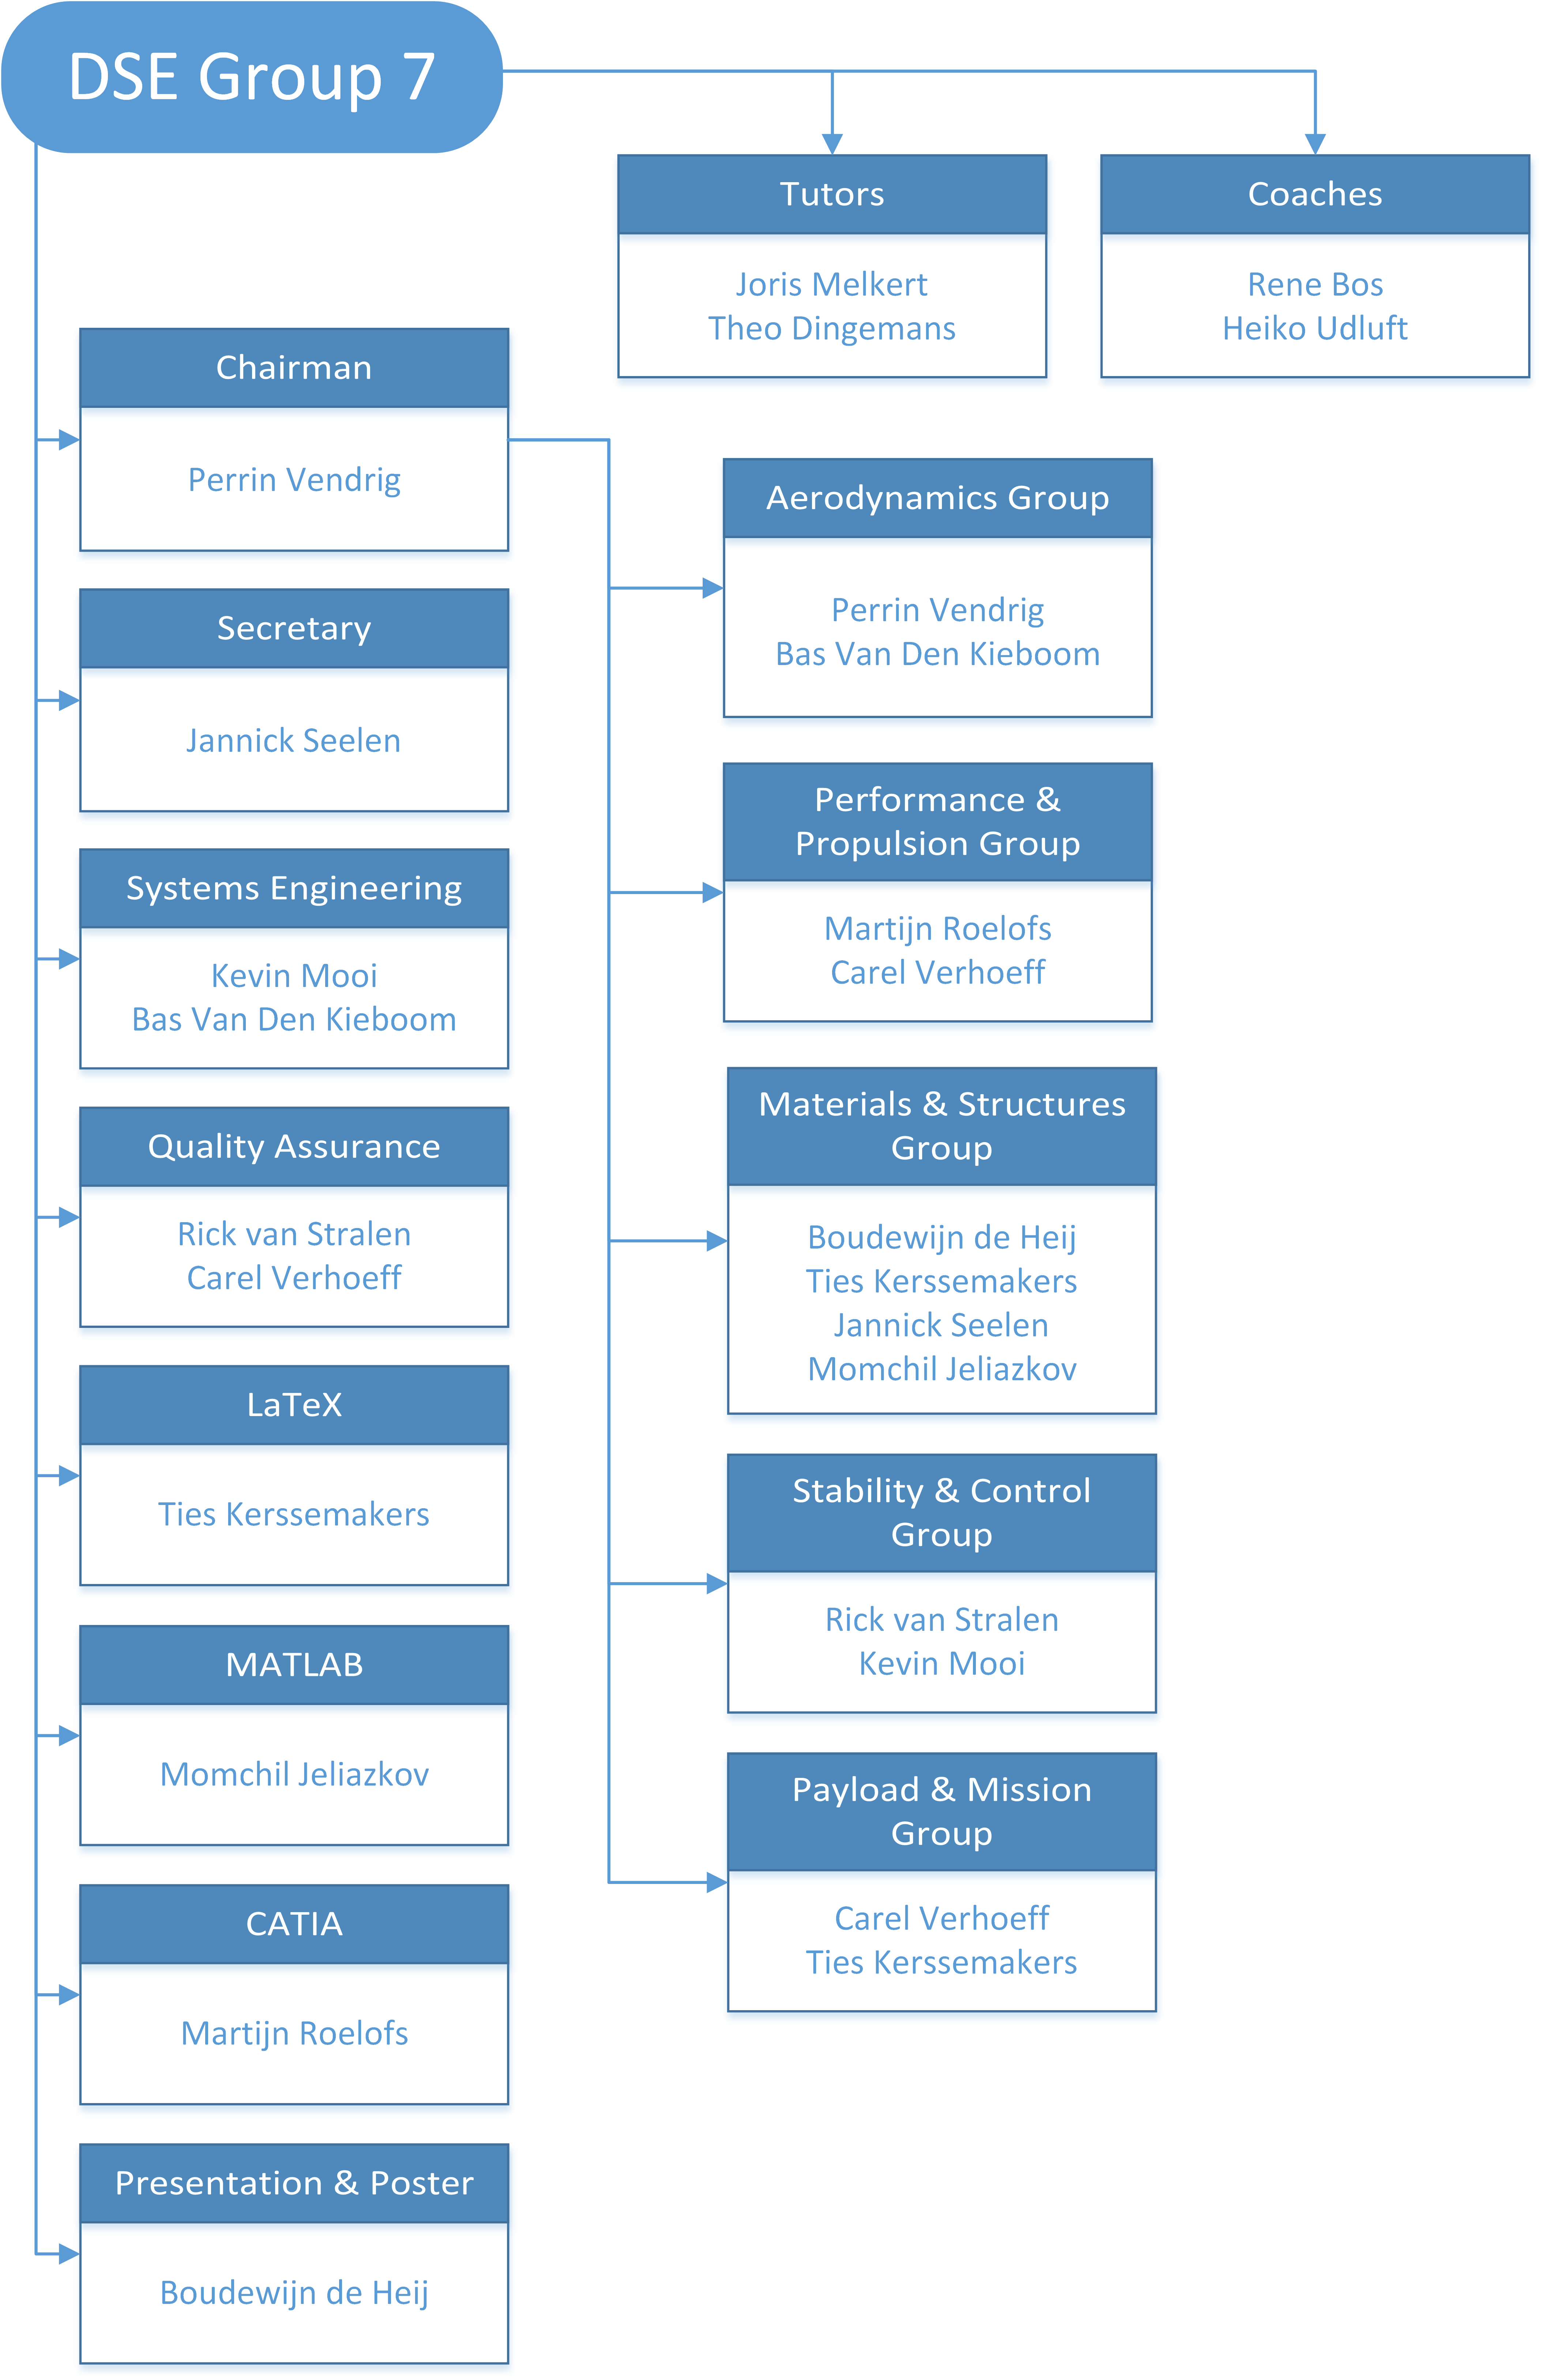
\includegraphics[width=0.6\textwidth]{Figures/Organogram2.png}
\caption{Organogram of the team organization}
\label{fig:Orgroles}
\end{figure}
\documentclass[a4paper]{report}
\usepackage[english]{babel}
\usepackage{amssymb}
\usepackage{amsmath}
\usepackage{graphicx}
\usepackage{float}
\usepackage{shortvrb}
\usepackage{cancel}
\usepackage[T1]{fontenc}
\usepackage{nicefrac}
\usepackage{amsfonts}
\usepackage{standalone} %Makes it possible to ignore other preambles of child document
\usepackage{eurosym} %Euro teken mogelijk
\usepackage{multirow} %For multiple rows togheter in one table
\usepackage{parskip} %For a small white line between paragraphs
\usepackage[protrusion=true,expansion=true]{microtype}
\usepackage{hyperref}%For automatic and URL Reference
\usepackage{appendix}
%Possible to change the margins
\usepackage{geometry}
\geometry{verbose,tmargin=1.9cm,bmargin=1.8cm,lmargin=2cm,rmargin=2cm}

\usepackage{subfig}

%include pdf pages
\usepackage{pdfpages}

%being able to create tables over multiple pages
\usepackage{longtable}

\makeatletter

%Change standard font size
\renewcommand\normalsize{ \@setfontsize\normalsize{11pt}{11pt}}\normalsize  
\makeatother

\usepackage{fancyhdr}
\pagestyle{fancy}
\fancyhead{}
\fancyfoot{}

%Gives text above each page
\fancyhead[CO,CE]{DSE Project}

%Page number
\fancyfoot[RO,LE]{\thepage}


\usepackage{babel}

%Available structures:
%Report: \part{}, \chapter{}, \section{}, \subsection{}, \subsubsection{}, \paragraph{}, \subparagraph{}


\begin{document}





\section{Control and monitoring the work}
To let the project run smoothly, some house rules and meetings are necessary. The house rules and meetings are needed to work as efficient as possible but also to create a good working environment. The house rules are:\\
\begin{itemize}
\item Follow the rules set by the DSE project and the Fellowship building.
\item Every day a logbook needs to be filled in by every member to specify what they did the past day during the working hours.
\item Every morning there is a brief meeting of 15 minutes.
\item Also weekly a meeting with the project mentors will be organized to give a status update and to have some time for questions from both students and mentors.
\item The working hours are from 9 am. till 5 pm.
\item Clean desk.
\item There is a lunch break of maximum 45 minutes each day.
\item When 15 minutes late one brings a cake next day.
\item Missing more than 2 hours at a particular day is considered a missed day.
\item All group stuff will be put in a locker at the end of the day.
\end{itemize}
The logbooks are needed to check what every member has been doing and if it takes too long to finish the part he is working on.\\
In the morning meetings a quick status update will be given and then is decided what should be done that day. During these meetings a status sheet will be filled in on how far the individual people are with their work. This status sheet will be filled in by the use of colours, green is the task is on schedule, yellow is a minor delay and red is a critical situation and the whole team must help. \\
The tutor meetings are needed to ask questions and to give a status update on how far the project has advanced. These meetings will take place once a week and the date will be planned with the tutors themselves. Before these meetings an agenda will be made to make the meeting as efficient as possible. The content of this agenda is determined during the weekly teammember meetings. At these weekly group meetings a summary will be made of the things that have been done so far.\\
If there is a delay by one of the group members or if deliverables can not be finished before the required deadlines, action should be taken. If one of the group members had an individual delay another group member can help or the one with the delay can finish it outside the project hour's. But if one of the deadlines is hard to complete the whole group should take action. These actions depend on the reason of the delay. The possible actions that can be taken are:
\begin{itemize}
\item Working outside the project hours.
\item Inform the tutors that it is impossible to deliver the report on time.
\item Decreasing the workload by leaving minor things out of the report and keep focus on the major issues.
\end{itemize}

\subsection{Version control}
Keeping track of changes and versions of project files is essential, especially for the reports, code files and CATIA. To keep this organized a SVN server is setup using virtualSVN server. A repository is installed on one team members' computer,  which acts as a server where the other members can update from and commit to. Using Version control programs such as tortoiseSVN on the client side makes it easy to commit one's changes and update the others'. Moreover, these tools provide merge options, to resolve possible conflicts. SVN has a changelog, in which each change is logged, with a message from the committer, the name of the committer, time/date and the affected files. The combination with the general logbook as well as the personal logbooks gives a clear view on the progress of the project. 
\end{document}


\end{document}
\documentclass[a4paper]{report}
\usepackage[english]{babel}
\usepackage{amssymb}
\usepackage{amsmath}
\usepackage{graphicx}
\usepackage{float}
\usepackage{shortvrb}
\usepackage{cancel}
\usepackage[T1]{fontenc}
\usepackage{hyperref}
\usepackage{epstopdf}
%Makes it possible to ignore other preambles of child document
\usepackage{standalone}

%Possible to change the margins
\usepackage{geometry}
\geometry{verbose,tmargin=1.9cm,bmargin=1.8cm,lmargin=2cm,rmargin=2cm}

\usepackage{subfig}

%include pdf pages
\usepackage{pdfpages}

%being able to create tables over multiple pages
\usepackage{longtable}

\makeatletter

%Change standard font size
\renewcommand\normalsize{ \@setfontsize\normalsize{11pt}{11pt}}\normalsize  

\makeatother

\usepackage{fancyhdr}
\pagestyle{fancy}
\fancyhead{}
\fancyfoot{}

%Gives text above each page
\fancyhead[CO,CE]{DSE Project}

%Page number
\fancyfoot[RO,LE]{\thepage}

\usepackage{babel}

%Available structures:
%Report: \part{}, \chapter{}, \section{}, \subsection{}, \subsubsection{}, \paragraph{}, \subparagraph{}

\begin{document}
\chapter{Schedule and Work Logic}
This chapter will document the planning at its current state for the entire project. The schedule is developed with the rolling wave principle in mind. Therefore the schedule below is presented in a detailed level up to the midterm report deadline and the schedule after that is only broadly planned. In order to be able to make a detailed planning, the project work-flow logic has to be considered simultaneously. Thus the work-flow logic will also be discussed in this chapter and the results will be presented in a Work-Flow Diagram (WFD). 

First the project milestones will be discussed, after which the project phasing will be presented. Since the phasing is also dependent on the work-flow logic, this will be discussed alongside it. The graphical results of these discussions will be presented in the form of a Gantt chart and Work-Flow Diagrams. Finally, the Work Breakdown Structure (WBS) diagram will also be shown, which is derived from the Gantt chart logic. Once the schedule has been discussed, some time will be spent to locate the scheduling risks.
\section{Milestones}
Three milestone reviews have been set. A Baseline Review (BR) is planned for May 6$^{th}$, a Midterm Review (MTR) is planned for May 30$^{th}$ and  the Final Review (FR) is planned for June 27$^{th}$. An additional milestone can be set for the DSE Symposium Day for July 4$^{th}$, at which point the results of the final Final Review have to be presented to a jury of experts. \newline

The deliverables for the Baseline Review are a Project Plan (PP) and the Baseline Report. The deliverables for the Midterm Review are a Midterm Report and the presentation of the results. For the Final Review the deliverables are the Final Report and a presentation on the results. Finally, for the Symposium a presentation and a poster need to be delivered. \newline

When developing the schedule, in general the deadlines for the milestones were used. The only exception is the Project Plan, which is due to be delivered on May 6$^{th}$. Internally the group has set a deadline for the Project Plan on April 26$^{th}$, in order to focus all the resources afterwards on the Baseline Report. 

\section{Project Phasing and Logic}
Now the milestones and deadlines are known, these can be used as a fixture to build the schedule around. The scheduling for each milestone will now be treated separately below. The Project Plan will be included with the Baseline Review milestone. 
\subsection{Baseline Review}
The first part of the Baseline Review concerns the Project Plan. Various tasks were defined in accordance to the deliverables listed in the Project Plan requirements. The task for Work Break-Down (WBS) structure was subdivided into the various specialty groups as defined in chapter \ref{Chapter:Teamorganization}. These specialty groups defined a more detailed work breakdown schedule once the general WBS was developed. Obviously the assignment of the human resources was dependent on the group organization, thus every task had to wait before this was completed. Once that was done, the work on the WBS, the Gantt chart and the Work-Flow Diagrams (WFD) could proceed in parallel. Finally, when this work was divided some spare human resources remained. These were assigned to perform the market analysis. \newline

The Gantt chart for the Project Plan and Baseline Review can be seen in \autoref{fig:ganttbr}. This figure shows the critical task of the Project Plan is the Gantt chart and the WFD.
%\thispagestyle{empty} 
\begin{figure}[h]
	\centering
	
	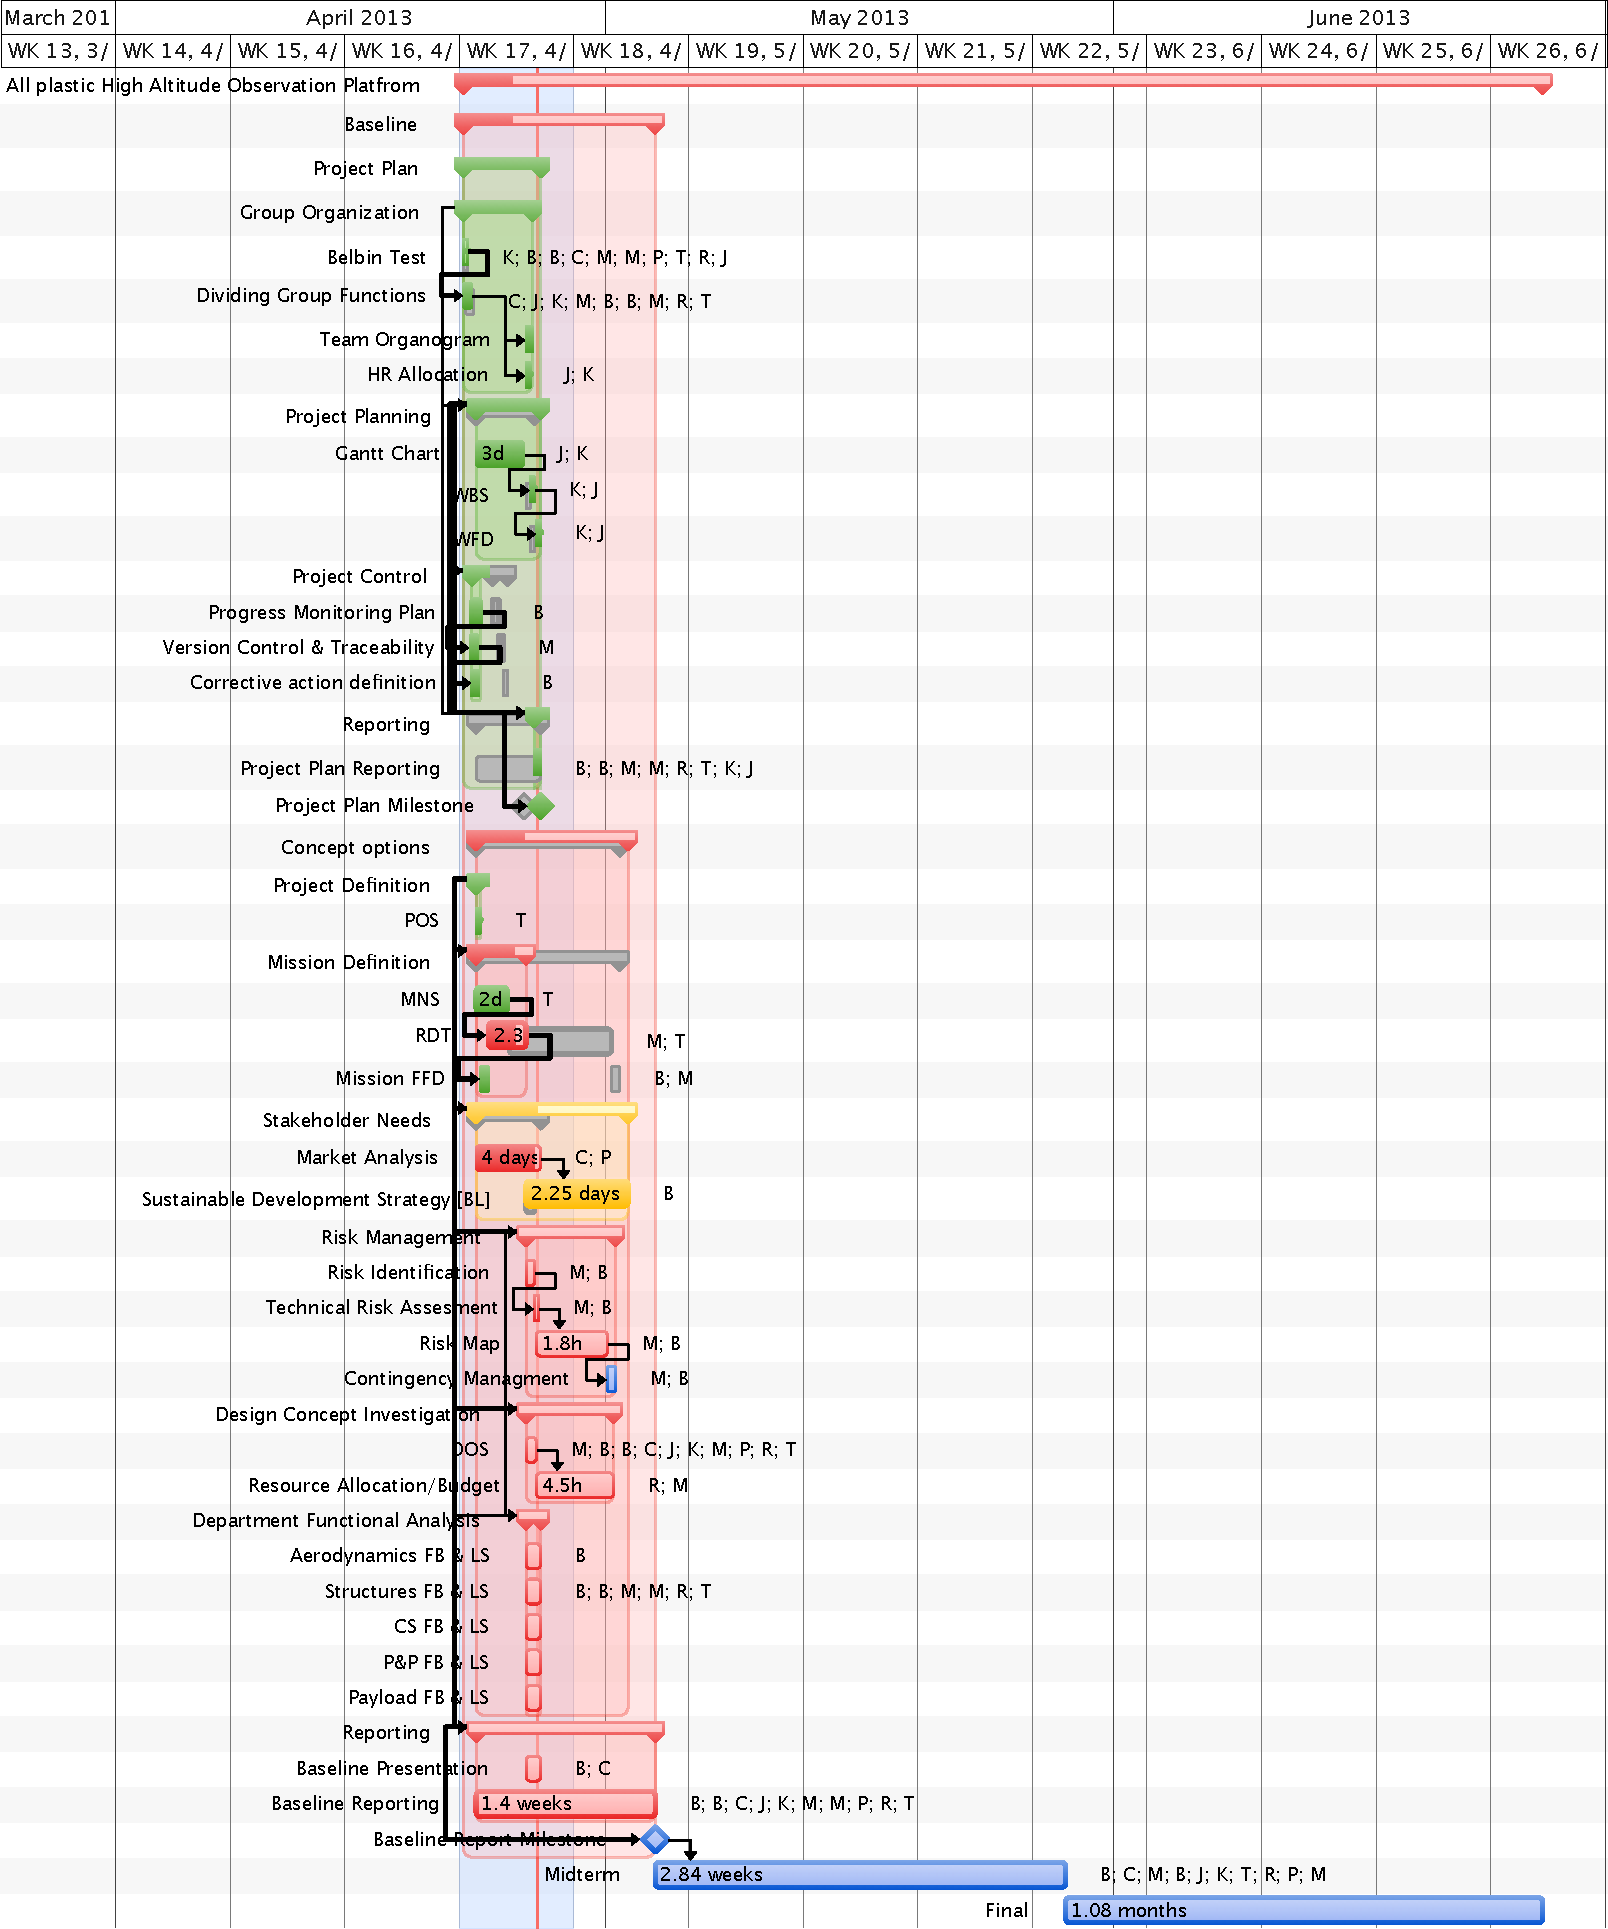
\includegraphics[width=\textheight, angle=270]{Figures/BASEGANTT.PDF}
	\caption{Gantt chart of the PP and BR schedule}
	\label{fig:ganttbr}
	
\end{figure}
The logical structure of the Gantt chart can be seen in \autoref{fig:wfdbr}. It can clearly be seen many of the tasks can be performed in parallel of each other. 

\subsection{Baseline Report}
\autoref{fig:ganttbr} also shows the Gantt chart for the Baseline Report planning. Apart from the deliverables specified, an extra task was added to the chart. A day is reserved for a literature study, to allow each specialist group to gain knowledge about the theory and the state of the art technology concerning their field. \newline

There are several dependencies between the various tasks, which means work needs to proceed in a more sequential fashion. Sustainable development strategy is linked to market analysis because sustainable development is becoming more and more a market driven requirement. The Requirement Discovery Tree needs to be  developed before a Design Option Structuring tree (DOS) can be made. The logic can be seen in \autoref{fig:wfdbr}.
\begin{figure}[h]
	\centering
	
	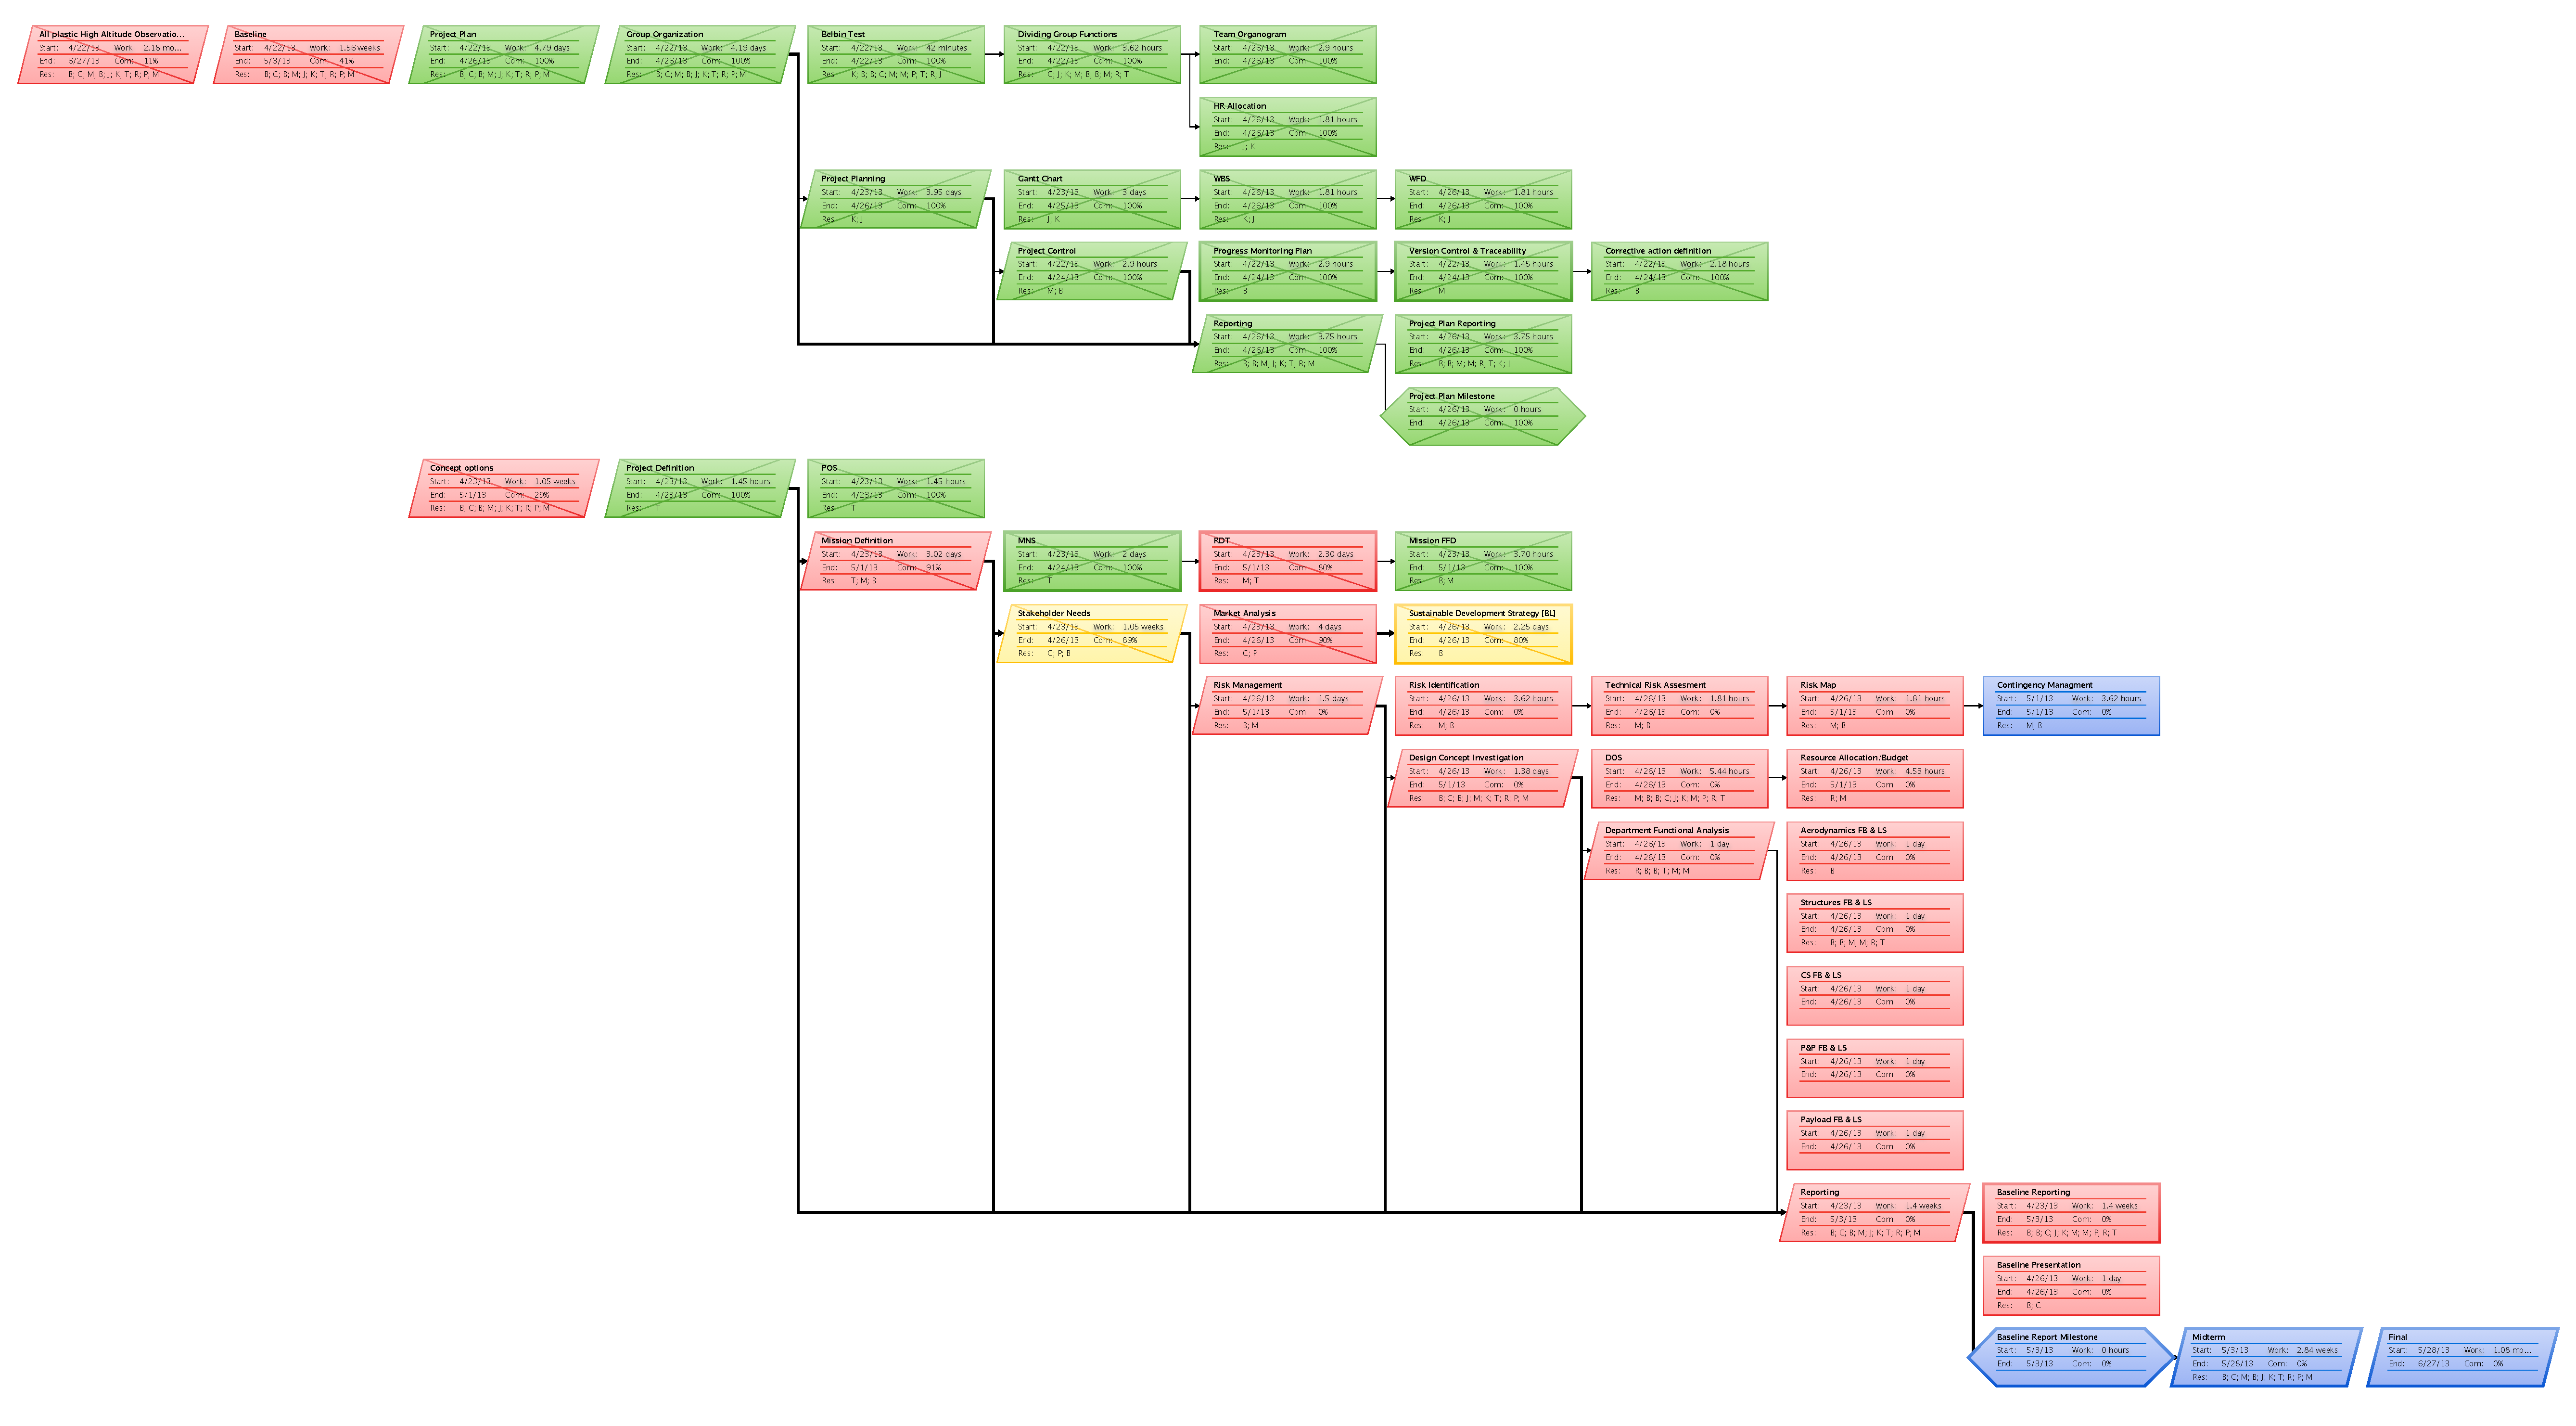
\includegraphics[width=\textwidth]{Figures/BASEWFD.pdf}
	\caption{WFD of the BR development}
	\label{fig:wfdbr}
	
\end{figure}
\subsection{Midterm Review}
During the midterm part of the project, five concepts will be chosen to further develop and evaluate. Once some predetermined data for these concepts is known, a trade-off can be performed to chose one final concept for further development. The Gantt chart for the Midterm review can be seen in \autoref{fig:ganttmtr}. 

\begin{figure}[h]
	\centering
	
	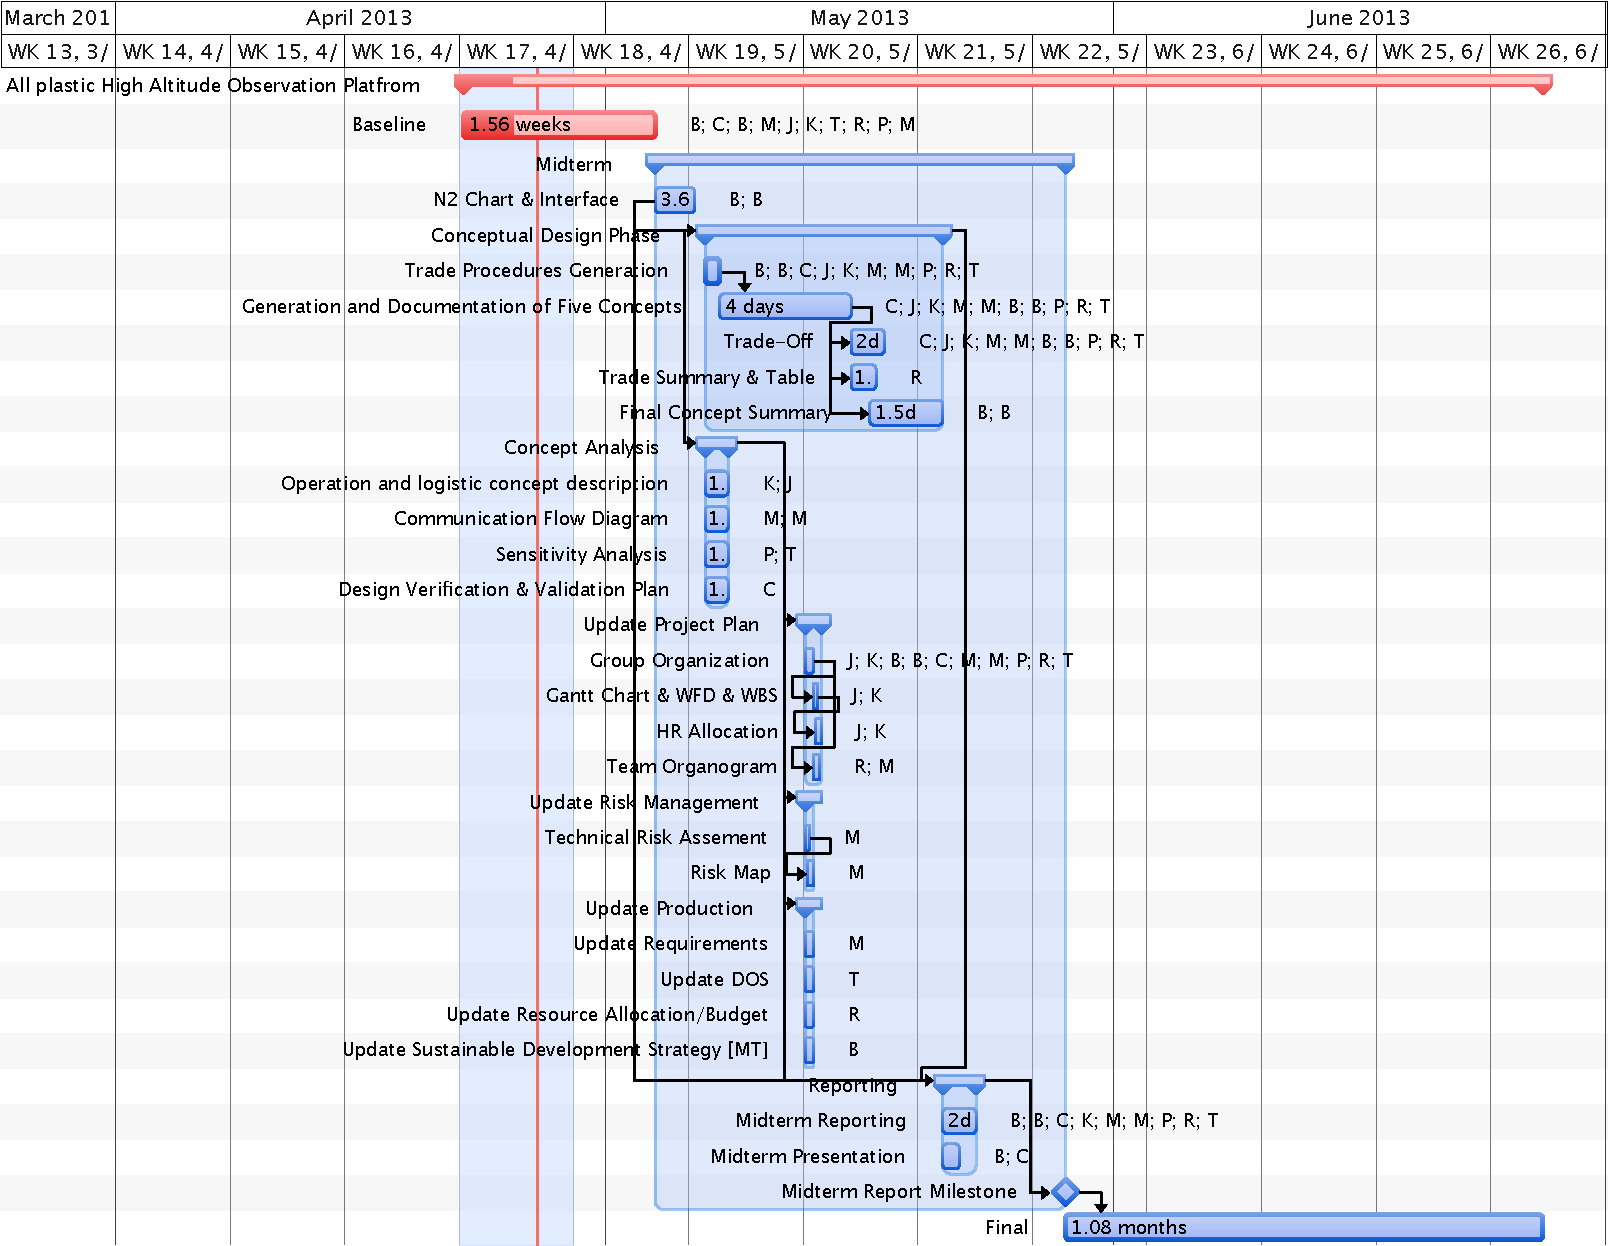
\includegraphics[width=\textheight, angle=270]{Figures/MIDGANTT.PDF}
	\caption{Gantt-chart for the development of the MTR}
	\label{fig:ganttmtr}
	
\end{figure}

First the entire group will agree on a trade method rationale and trade criteria. Then the group is split in five groups of two, which each develop a promising concept and generate some data for the previous set criteria. Once this is done, the group comes back together and chooses a final concept. Some analysis is subsequently performed on this concept, such as an operation and logistic investigation and a sensitivity analysis. Finally, a number of documents such as the risk assessment and Gantt chart will be updated at the end of this phase. The entire work-flow logic can be seen in \autoref{fig:wfdmtr}. 
\begin{figure}[h]
	\centering
	
	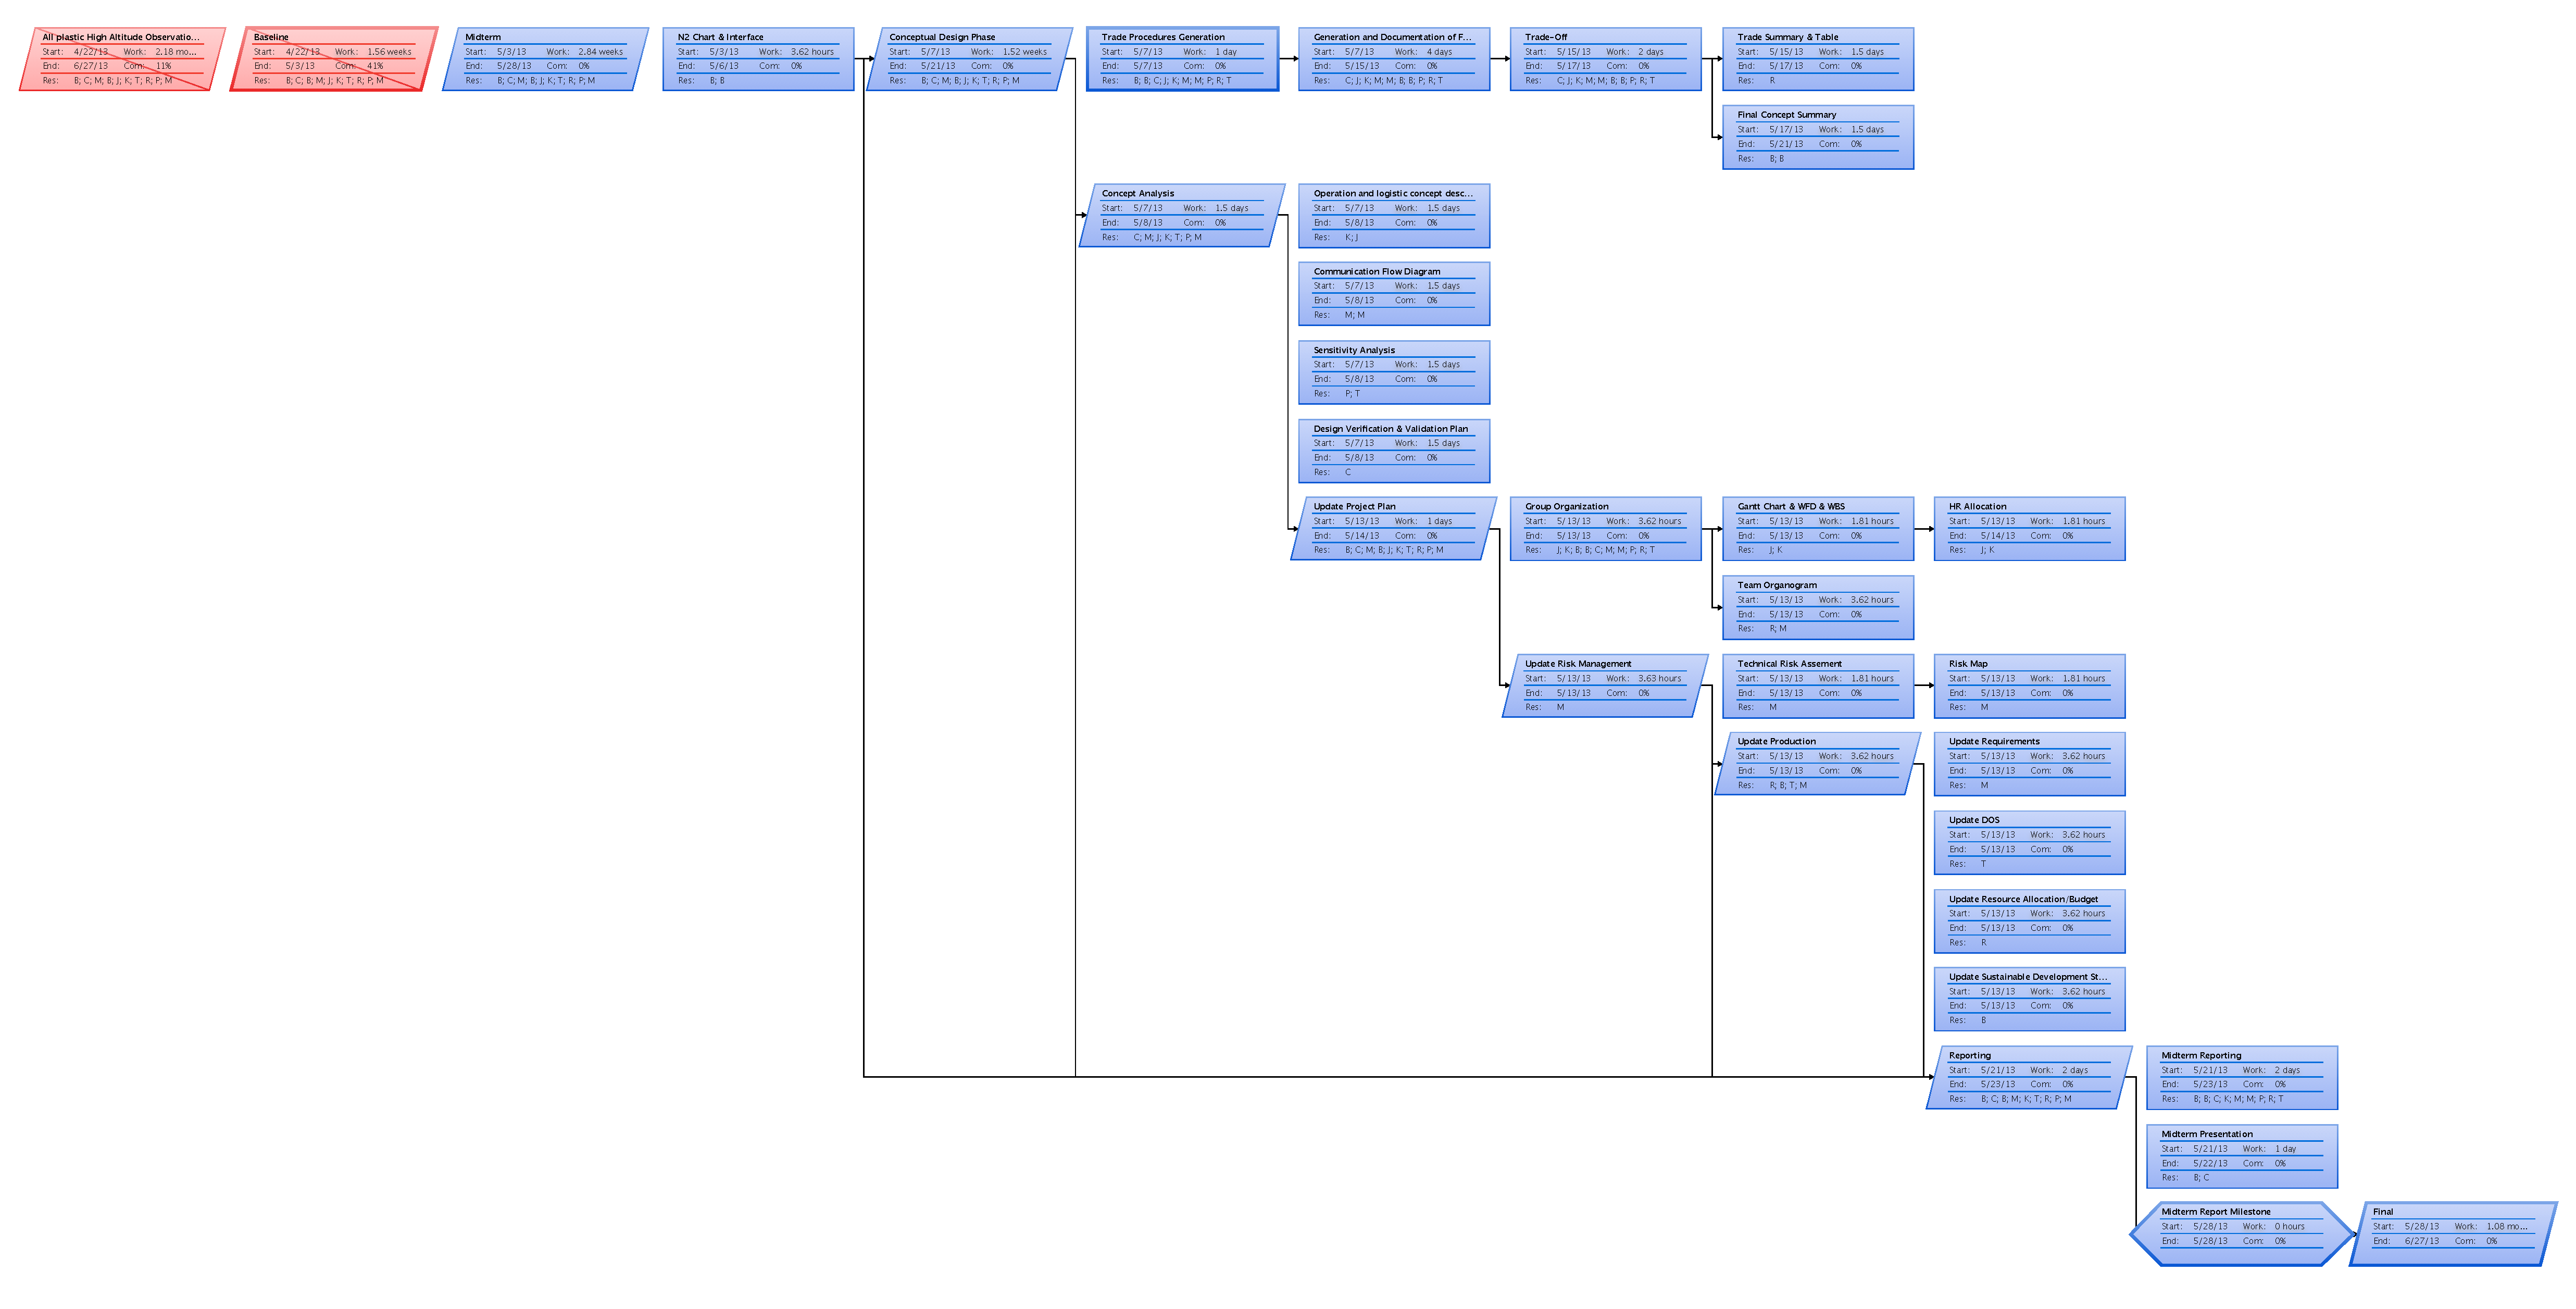
\includegraphics[width=\textwidth]{Figures/MIDWFD.pdf}
	\caption{WFD of the MTR development}
	\label{fig:wfdmtr}
	
\end{figure}

\subsection{Final Review}
A Gantt chart and Work-Flow Diagram were also created for a the Final Review. The schedule is very uncertain for this part of the project, therefore no further elaboration is given here. The charts can be seen in \autoref{fig:ganttfr} and \autoref{fig:wfdfr}.
\begin{figure}[h]
	\centering
	
	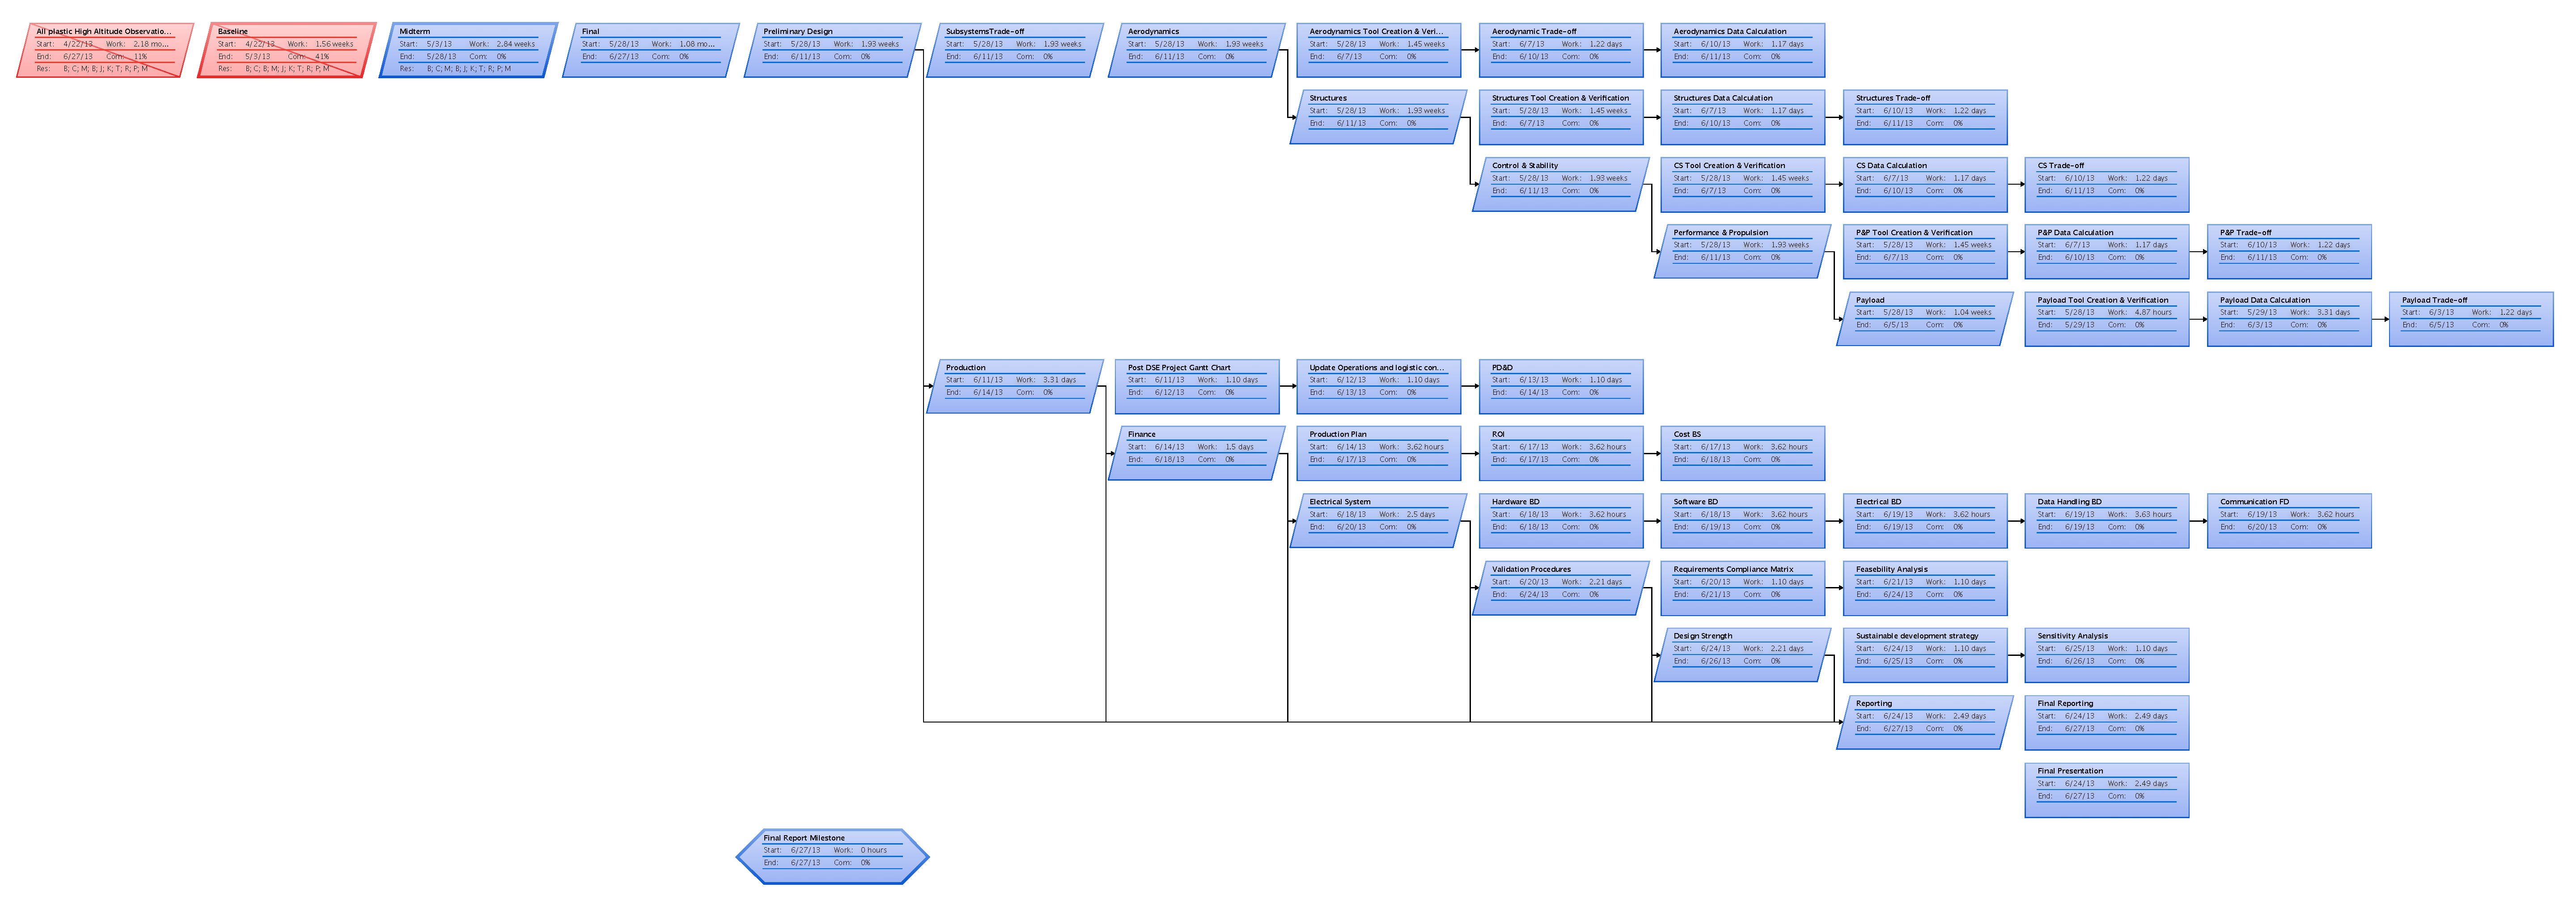
\includegraphics[width=\textwidth]{Figures/FINALWFD.pdf}
	\caption{WFD of the FR development}
	\label{fig:wfdfr}
	
\end{figure}
\begin{figure}[h]
	\centering
	
	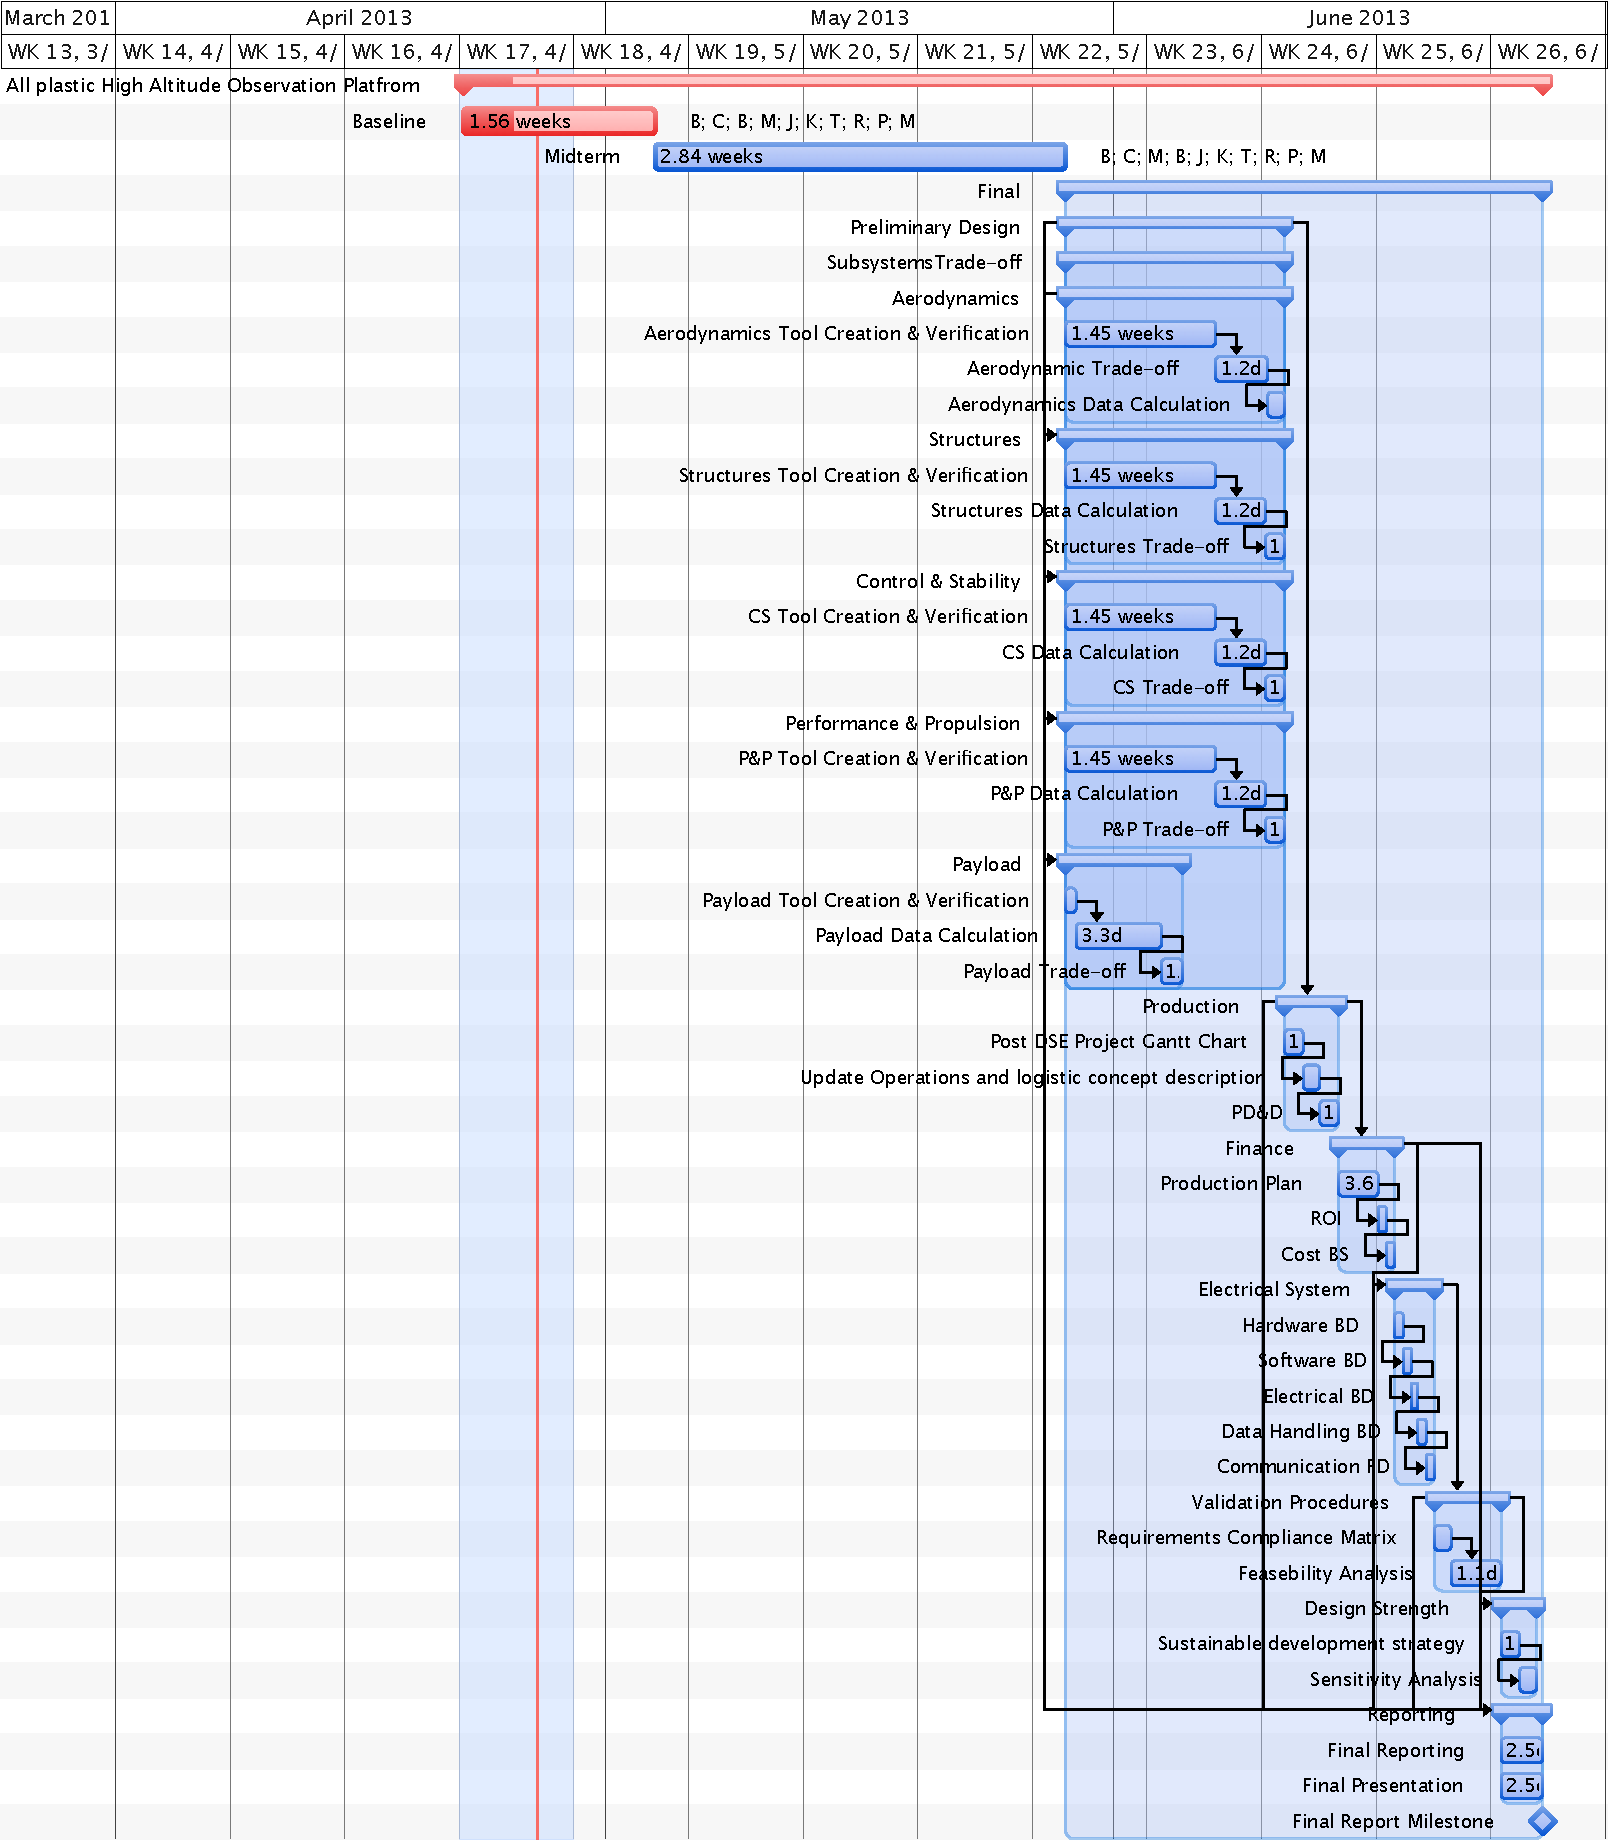
\includegraphics[width=\textwidth]{Figures/FINALGANTT.pdf}
	\caption{Gantt Chart for the Final Review}
	\label{fig:ganttfr}
	
\end{figure}

\section{Work Breakdown Structure}
The Work Breakdown Structure presents the structure of the entire project in a hierarchical tree and can be seen in \autoref{fig:wbs}. The data for this structure was taken from the Gantt chart. Final review is included in the structure, however little is certain about this part of project and it can be expected this part will change in the future.  

\begin{figure}[h]
	\centering
	
	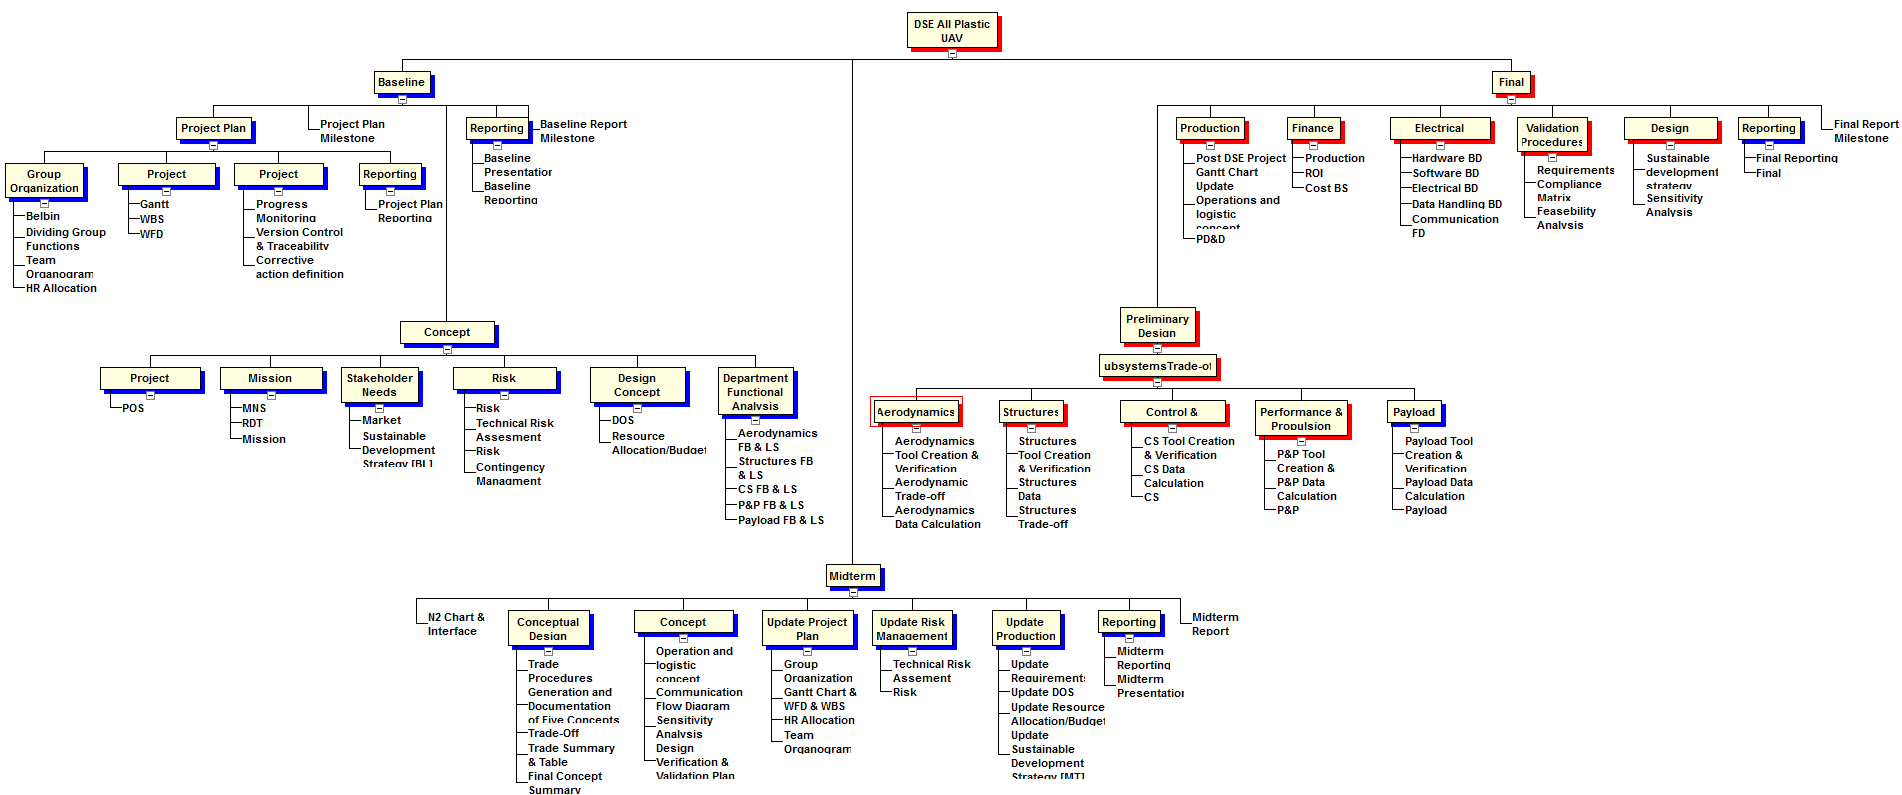
\includegraphics[width=\textheight, angle=270]{Figures/WBS.png}
	\caption{WFD of the MTR development}
	\label{fig:wbs}
	
\end{figure}
\section{Schedule Risk}
This sub-chapter will briefly discuss the risk associated with the schedule up to the Midterm Review. The risk associated with planning for the Final Review will not be discussed, since it is far into the future and little is known about it at this stage of the project. Thus any discussion regarding associated risk will be meaningless. 
\subsection{Baseline Milestone Risk}
When looking at the schedule for the Baseline Review, it can be seen there is no room for slack planned in at all. Even worse, the presentation is actually scheduled to be completed after the milestone. This is possible because the presentation is not part of the report, but of the review which has a slightly later deadline. 
\newline
Zero slack is a big risk. If any critical task is delayed, the milestone will not be met. It is a highly undesirable situation, but cannot be avoided at this point in time due to short period up to the deadline. The consequence is the planning needs to be vigilantly guarded. When it is not met, extra work has to be put in to ensure schedule compliance.
\subsection{Midterm Milestone Risk}
Unlike the Baseline Milestone, the schedule for the Midterm milestone contains considerable slack. Since this is a design phase, it can be expected tasks will take longer than anticipated. This was also emphasized during a discussion with one of the coaches. 
\newline
The risk for delay to the Midterm Milestone is difficult to quantify at this stage. It is estimated it will be lower compared to the Baseline Report Risk. 

\end{document}


\documentclass[a4paper]{report}
\usepackage[english]{babel}
\usepackage{amssymb}
\usepackage{amsmath}
\usepackage{graphicx}
\usepackage{float}
\usepackage{shortvrb}
\usepackage{cancel}
\usepackage[T1]{fontenc}
\usepackage{nicefrac}
\usepackage{amsfonts}
\usepackage{standalone} %Makes it possible to ignore other preambles of child document
\usepackage{eurosym} %Euro teken mogelijk
\usepackage{multirow} %For multiple rows togheter in one table
\usepackage{parskip} %For a small white line between paragraphs
\usepackage[protrusion=true,expansion=true]{microtype}
\usepackage{hyperref}%For automatic and URL Reference
\usepackage{appendix}
%Possible to change the margins
\usepackage{geometry}
\geometry{verbose,tmargin=1.9cm,bmargin=1.8cm,lmargin=2cm,rmargin=2cm}

\usepackage{subfig}

%include pdf pages
\usepackage{pdfpages}

%being able to create tables over multiple pages
\usepackage{longtable}

\makeatletter

%Change standard font size
\renewcommand\normalsize{ \@setfontsize\normalsize{11pt}{11pt}}\normalsize  
\makeatother

\usepackage{fancyhdr}
\pagestyle{fancy}
\fancyhead{}
\fancyfoot{}

%Gives text above each page
\fancyhead[CO,CE]{DSE Project}

%Page number
\fancyfoot[RO,LE]{\thepage}


\usepackage{babel}

%Available structures:
%Report: \part{}, \chapter{}, \section{}, \subsection{}, \subsubsection{}, \paragraph{}, \subparagraph{}

\begin{document}
\chapter{Sustainable development approach}
\label{Sustainable development approach}
In current social climate it is more and more important to develop in a sustainable way. Sustainable development is defined in the Brundtland report\cite{brundtland1987}, quoting:\\
\textit{''Sustainable development is development that meets the needs of the present without compromising the ability of future generations to meet their own needs.''}\\
Sustainable development is achieved by looking at the whole life cycle of the product, reducing unnecessary expenses, use of material and energy as well  as reducing the thrown away material. Also reusing materials will help.\\
For the All plastic High Altitude Observation platform the complete life cycle is taken into account. The main goals are cheap sustainable production and a long life time cycle. A long lifetime gives a high efficiency of the production stage. The advantage of an all plastic vehicle is that a long life time can be achieved by using wear resistant materials. Furthermore a wide variety of plastics can be produced easily, in contrast with metals and metal alloys. The production techniques of these materials require low amount of material.\\ 
With battery technology improvement the amount of energy stored per weight is growing fast. This allows light weight batteries, using less material. Current developments in polymer solar panels are promising. Production of polymer solar panels can be much cleaner than the production of current solar panels. Currently used solar panels contain high amounts of rare metals such as galium, indium and selenium. Mining and production of rare metals is a polluting industry. Also the available amount of these rare earth elements is reducing\cite{website:discovery.com1}\cite{website:phys.org1} and therefore it is a good development to have alternative methods for energy production and storage.\\
Another approach of the sustainable development of the observation platform will be 3D printing. 3D printing is a production method that allows cheap and fast production of plastic structures.  There is no excess material after printing parts. Connections can be made without riveting, while gluing or other connection techniques can be minimized. This can reduce the weight which reduces the required material, energy of production and energy during operation. Due to the relatively cheap  production the product becomes available to a wider public.\\
During the operational life of the aircraft, sustainability is important. Which energy source is used for continued flight can have a big impact on the environment. The use of natural sources with low emission of green house gasses or other harmful materials is preferred over polluting propulsion. A good example is solar power over jet fuel as an energy source.


\end{document}
\newpage
\bibliographystyle{aiaa}
\bibliography{Bibliography/bibliography}

\begin{appendices}
%\documentclass[a4paper]{report}
\usepackage[english]{babel}
\usepackage{amssymb}
\usepackage{amsmath}
\usepackage{graphicx}
\usepackage{float}
\usepackage{shortvrb}
\usepackage{cancel}
\usepackage[T1]{fontenc}
\usepackage{nicefrac}
\usepackage{amsfonts}
\usepackage{standalone} %Makes it possible to ignore other preambles of child document
\usepackage{eurosym} %Euro teken mogelijk
\usepackage{multirow} %For multiple rows togheter in one table
\usepackage{parskip} %For a small white line between paragraphs
\usepackage[protrusion=true,expansion=true]{microtype}
\usepackage{hyperref}%For automatic and URL Reference
\usepackage{appendix}
%Possible to change the margins
\usepackage{geometry}
\geometry{verbose,tmargin=1.9cm,bmargin=1.8cm,lmargin=2cm,rmargin=2cm}

\usepackage{subfig}

%include pdf pages
\usepackage{pdfpages}

%being able to create tables over multiple pages
\usepackage{longtable}

\makeatletter

%Change standard font size
\renewcommand\normalsize{ \@setfontsize\normalsize{11pt}{11pt}}\normalsize  
\makeatother

\usepackage{fancyhdr}
\pagestyle{fancy}
\fancyhead{}
\fancyfoot{}

%Gives text above each page
\fancyhead[CO,CE]{DSE Project}

%Page number
\fancyfoot[RO,LE]{\thepage}


\usepackage{babel}

%Available structures:
%Report: \part{}, \chapter{}, \section{}, \subsection{}, \subsubsection{}, \paragraph{}, \subparagraph{}

\begin{document}
\chapter{Work breakdown structure}

\begin{figure}
\label{fig:WBSFPP}
\centering
\includegraphics[height=20cm]{Figures/WBS_FPP.png}
\caption{performance and propulsion WBS tree}
\end{figure}

\begin{figure}
\label{fig:WBSA}
\centering
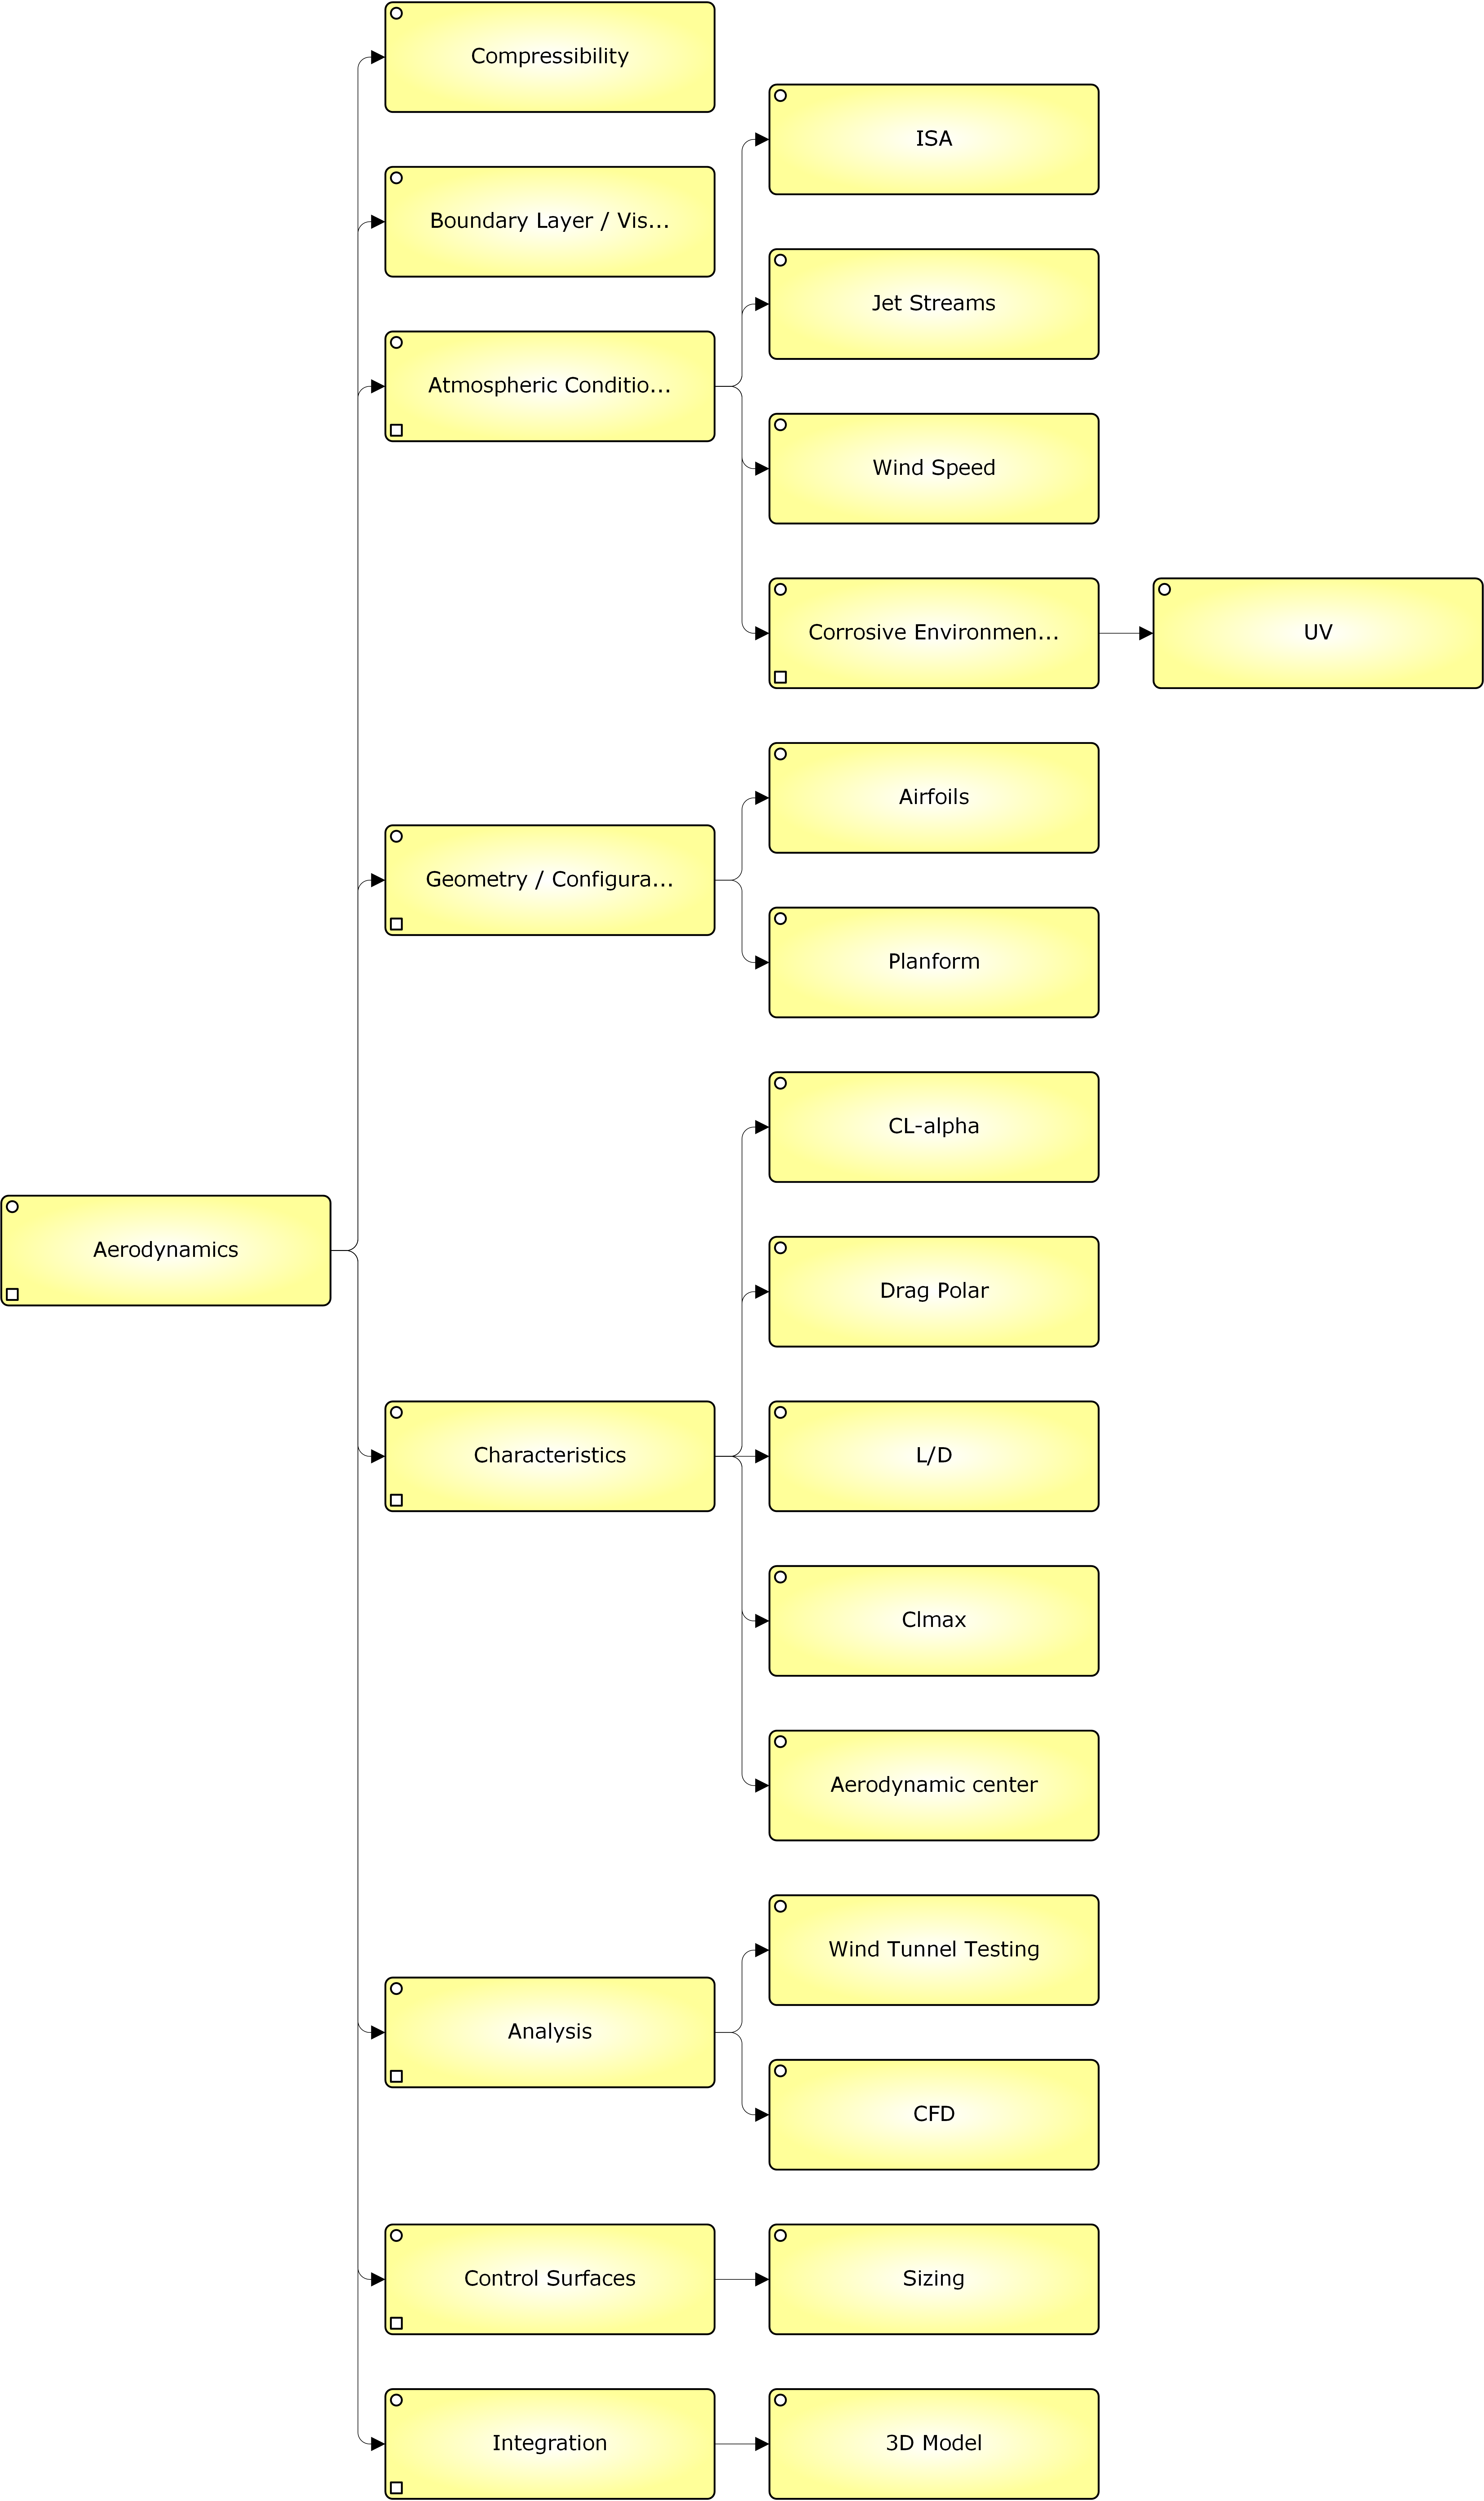
\includegraphics[height=20cm]{Figures/WBS_A.png}
\caption{Aerodynamics WBS tree}
\end{figure}



\begin{figure}
\label{fig:WBSSC}
\centering
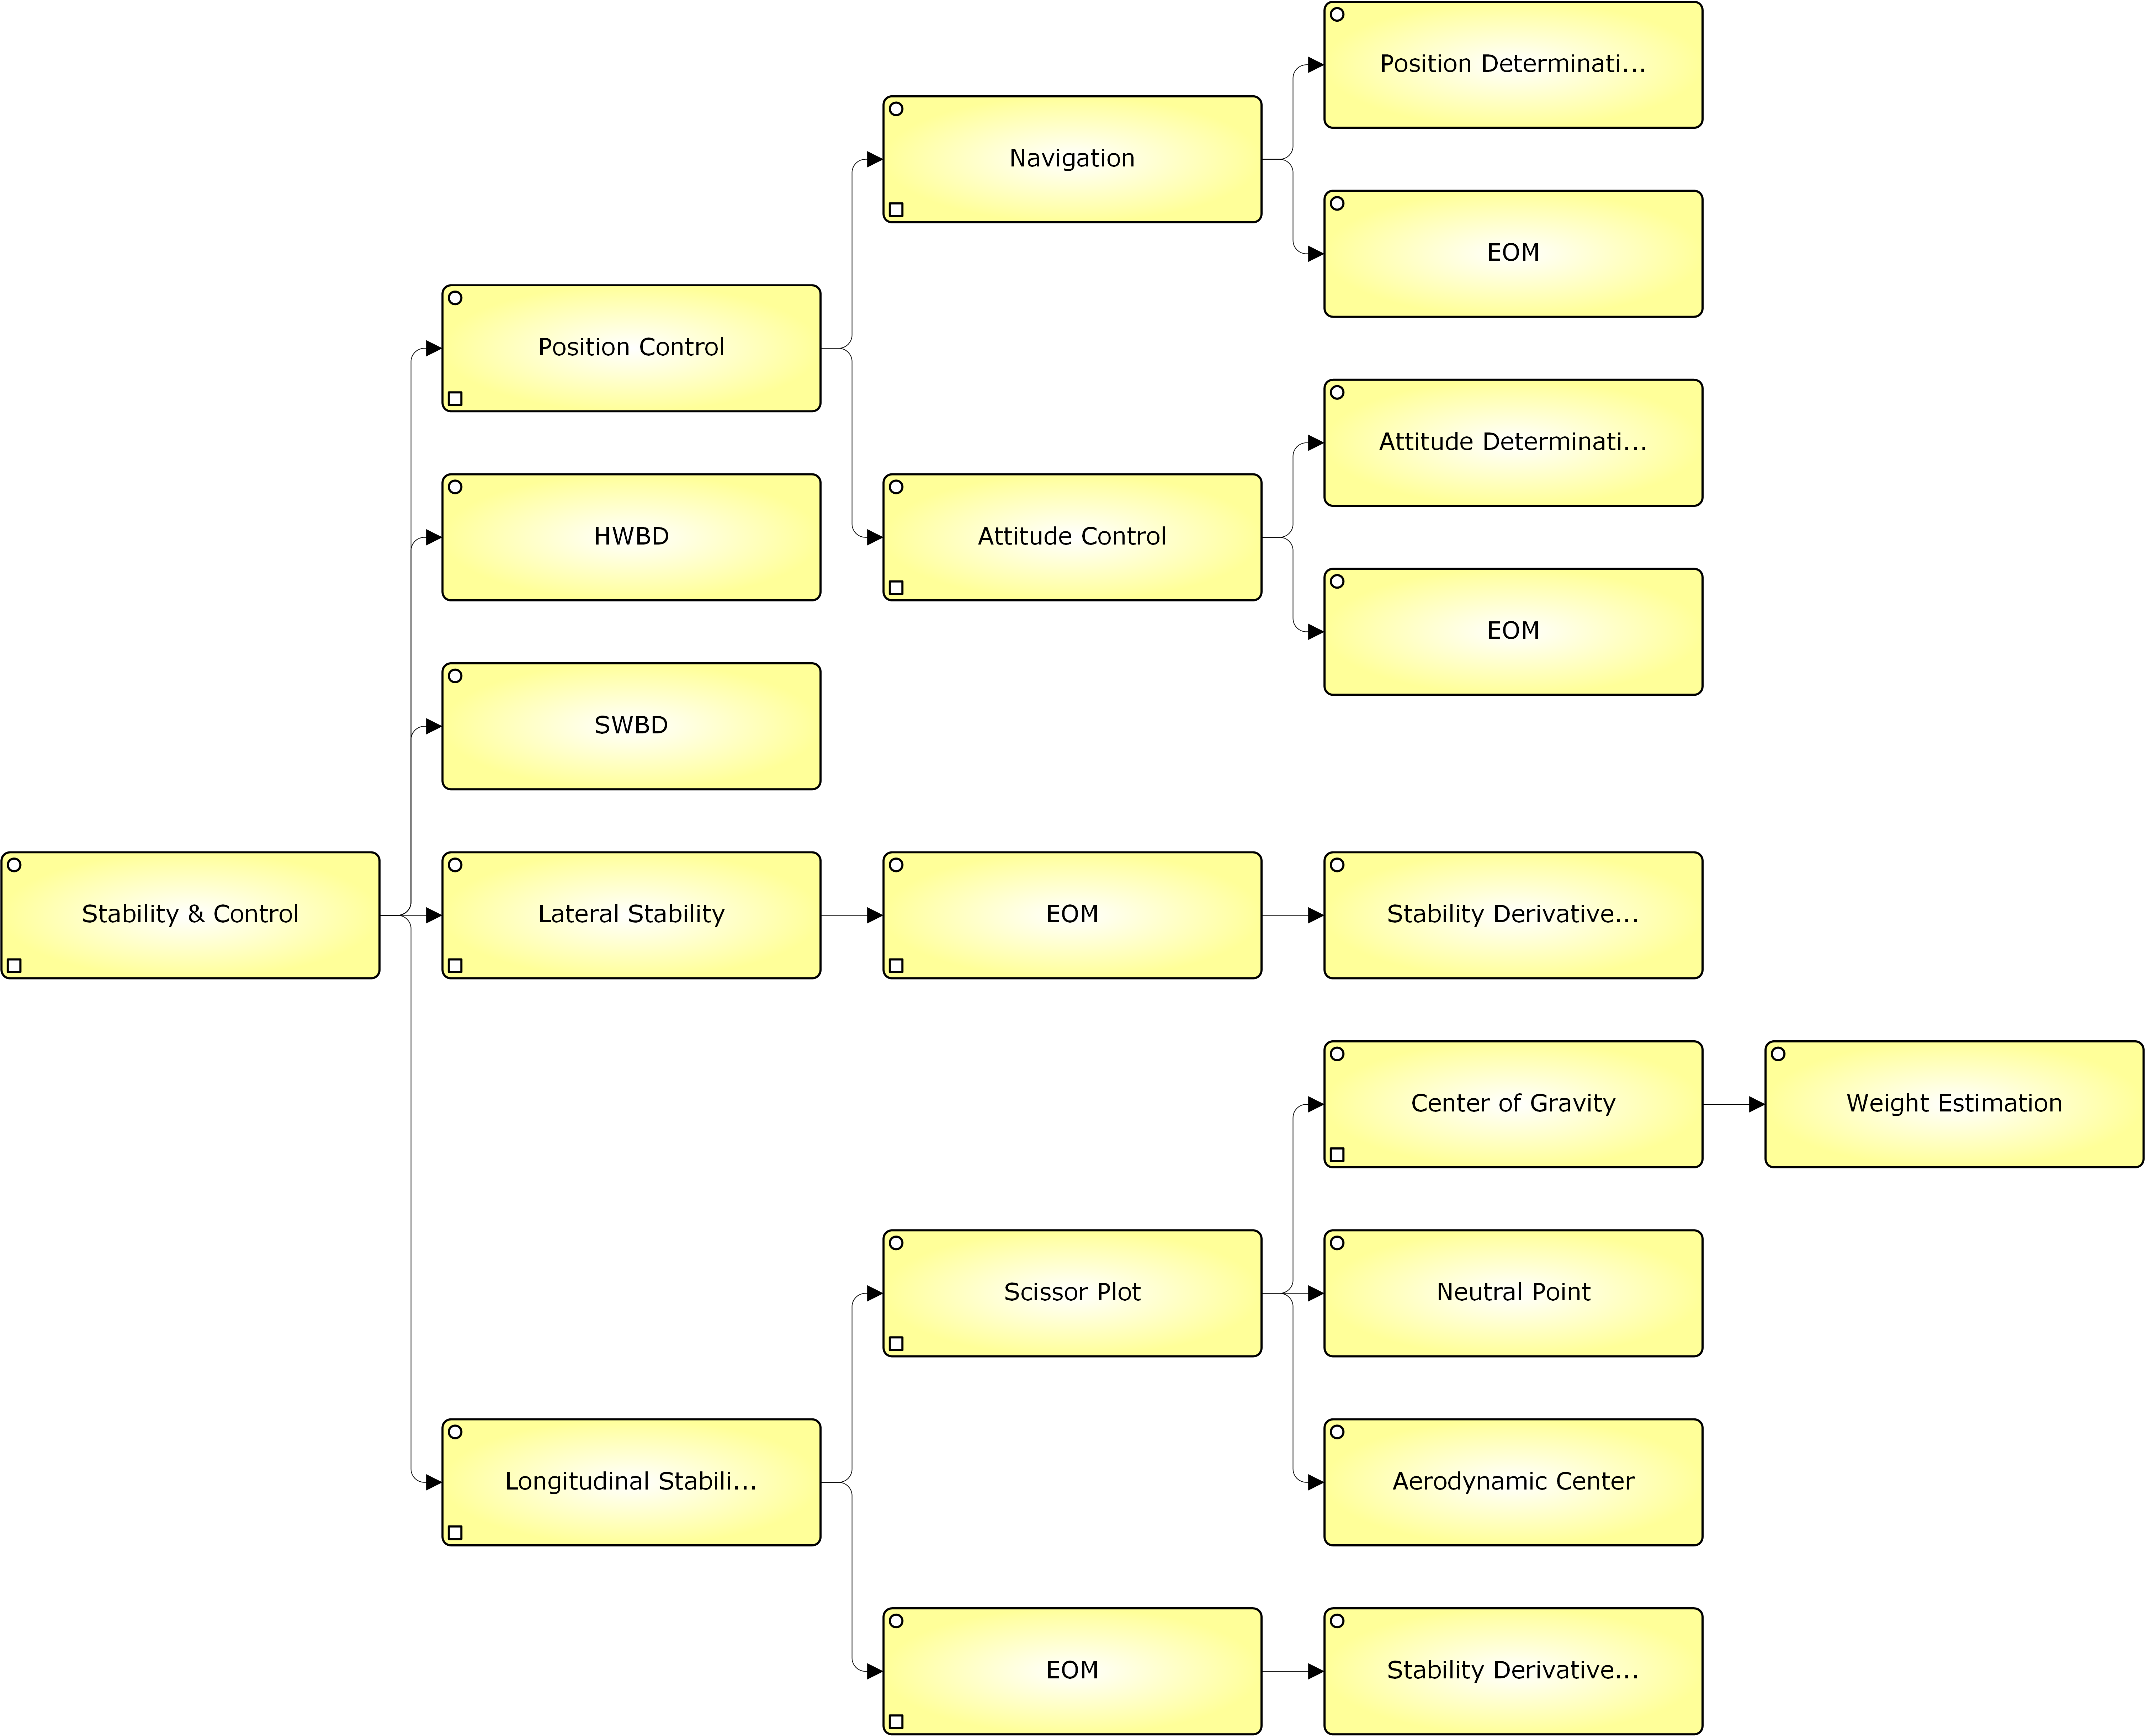
\includegraphics[width=\textwidth]{Figures/WBS_SC.png}

\caption{Stability and control WBS tree}
\end{figure}


\begin{figure}
\label{fig:WBSMS}
\centering
\includegraphics[height=20cm]{Figures/WBS_MS.png}

\caption{Materials and structural WBS tree}
\end{figure}



\begin{figure}
\label{fig:WBSPM}
\centering
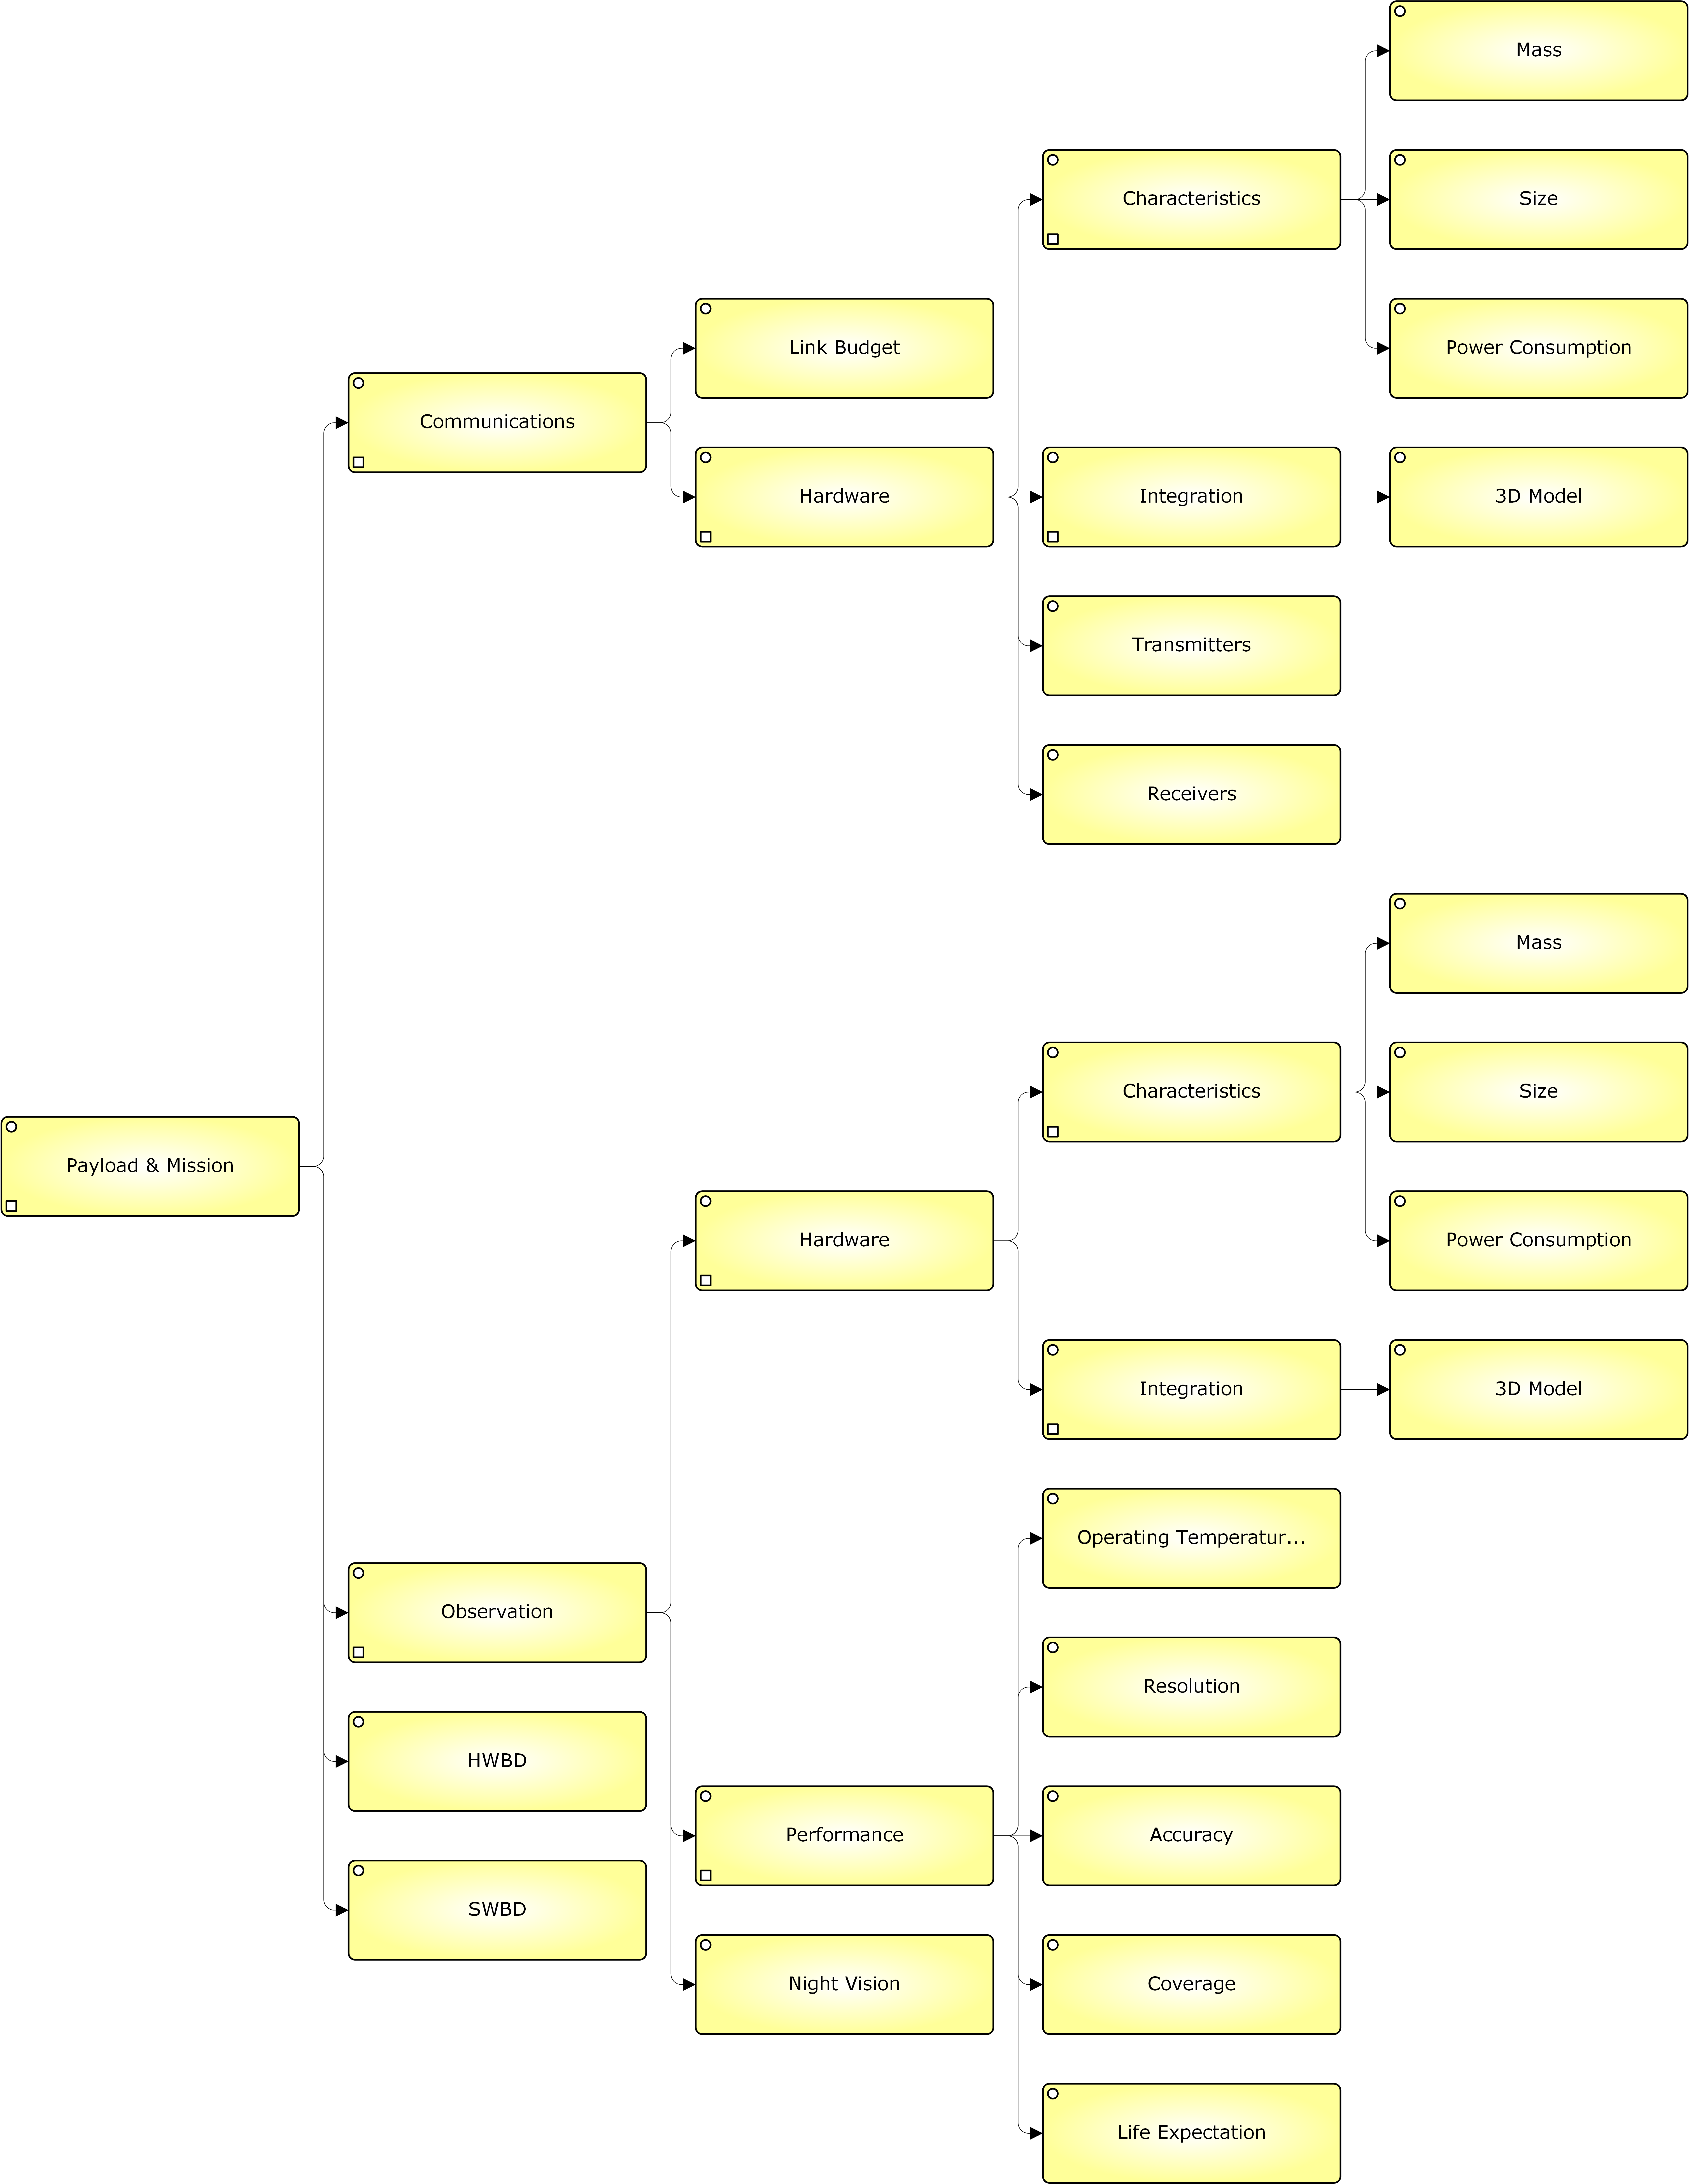
\includegraphics[height=20cm]{Figures/WBS_PM.png}

\caption{Payload and mission WBS tree}
\end{figure}


\begin{figure}
\label{fig:WBSO}
\centering
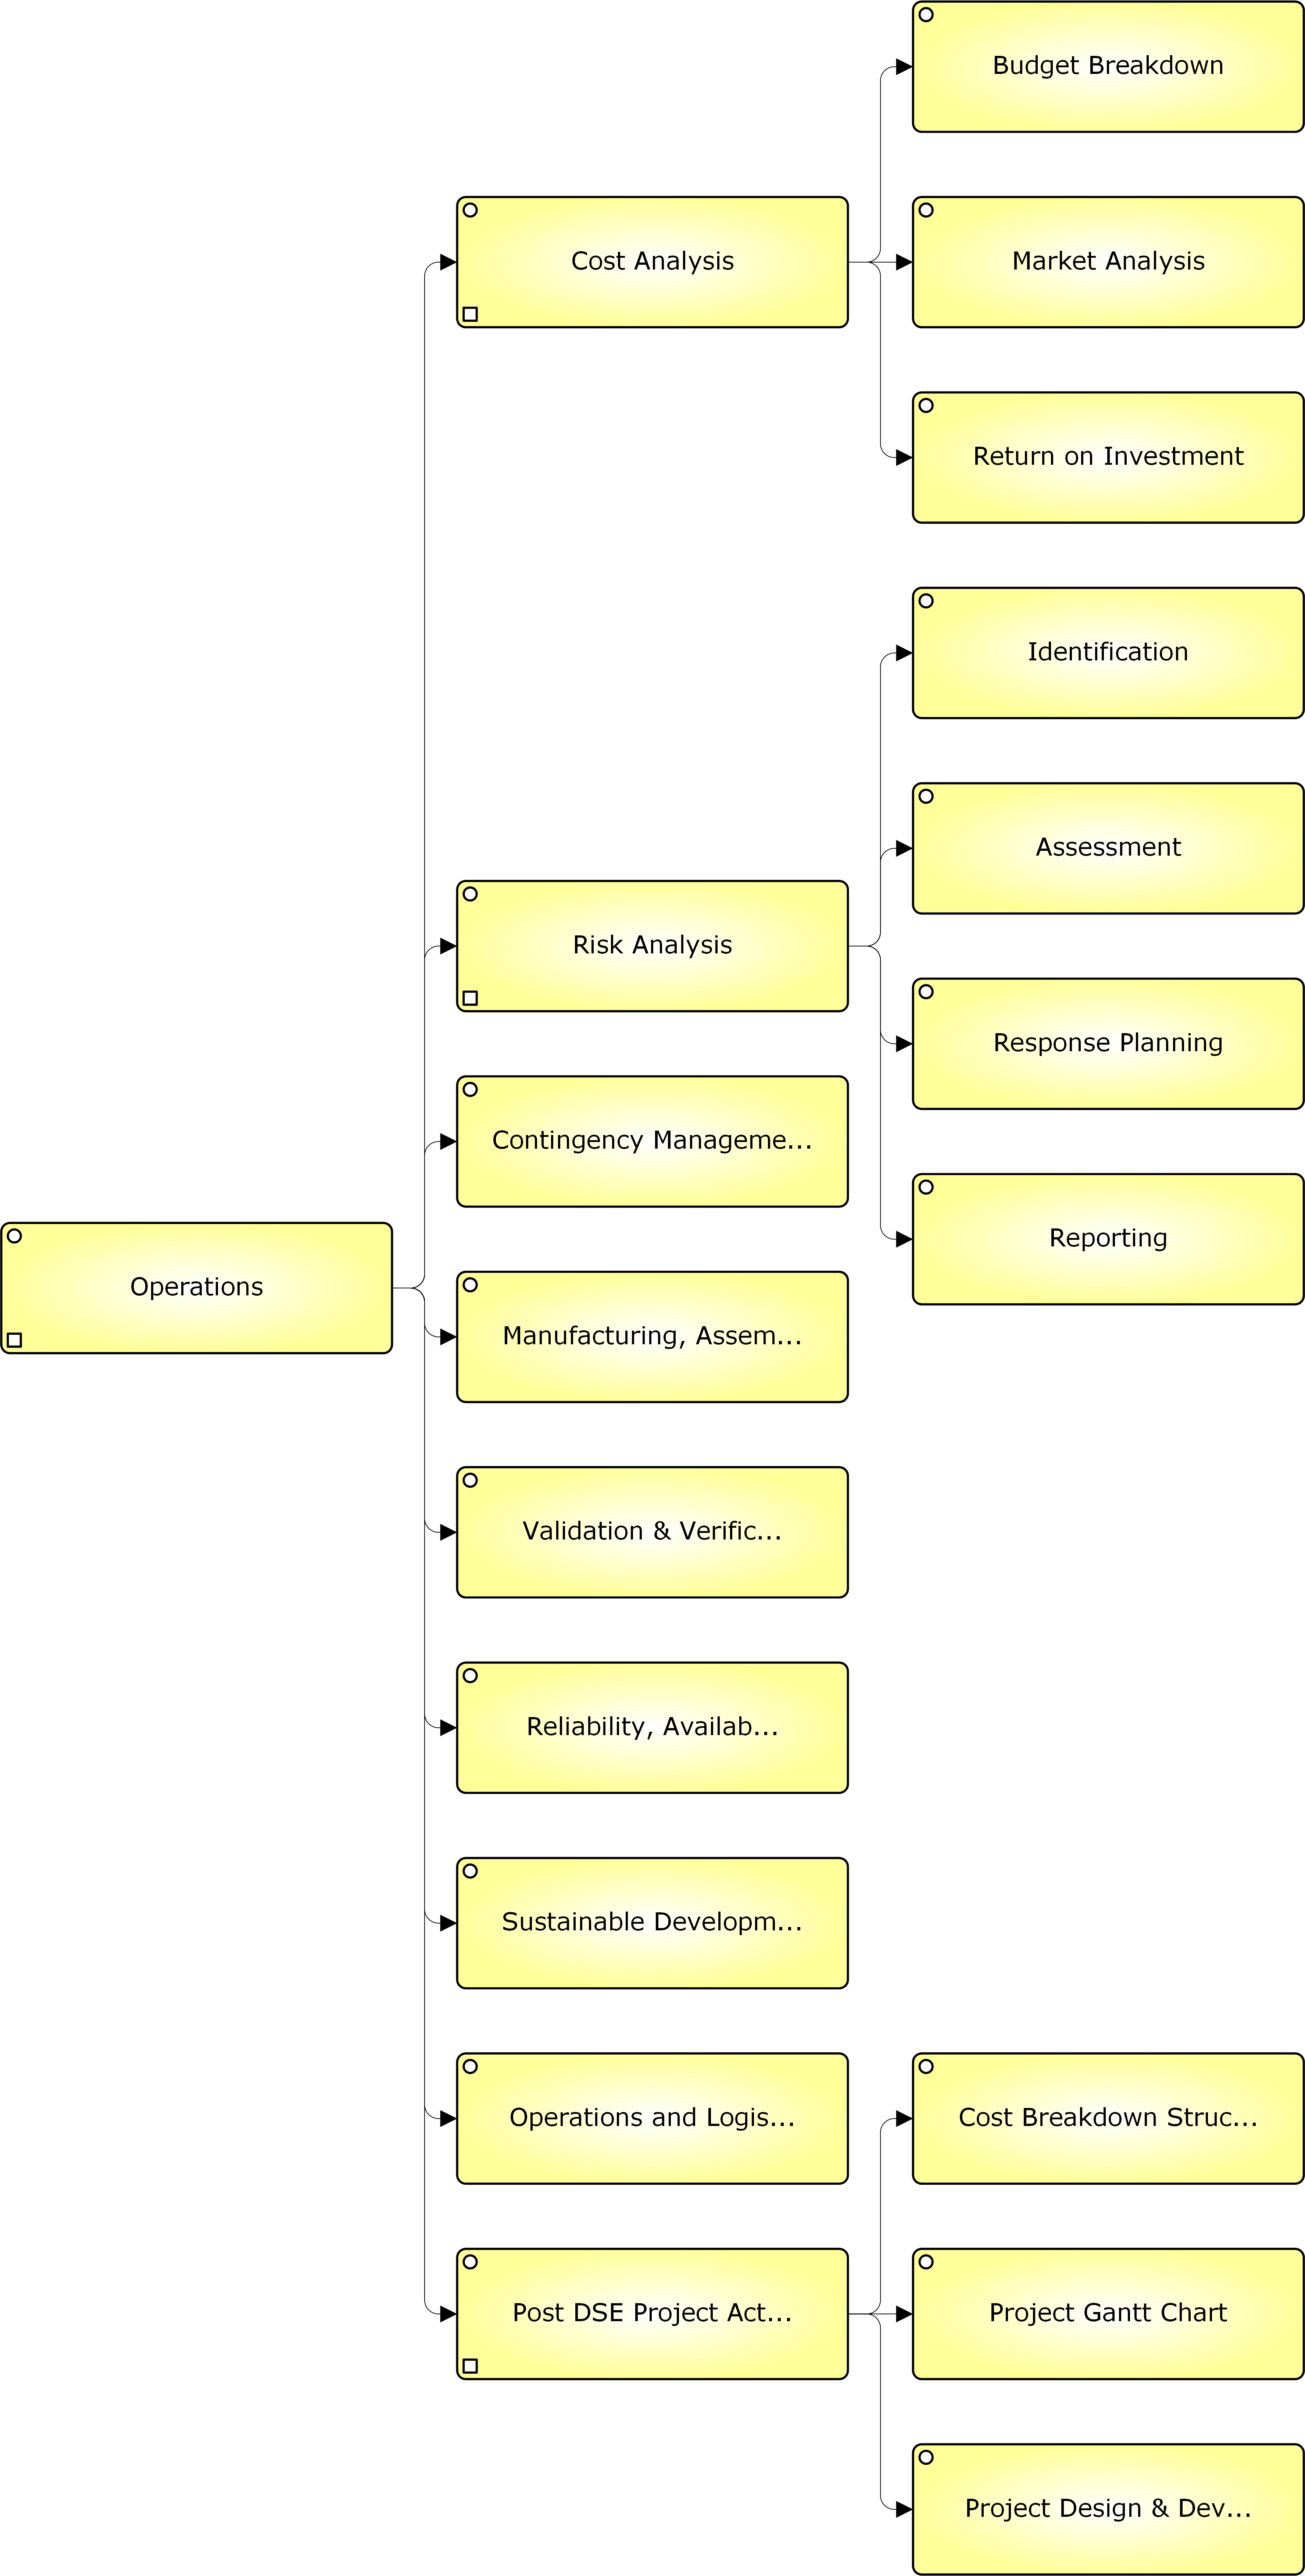
\includegraphics[height=20cm]{Figures/WBS_O.png}

\caption{operations WBS tree}
\end{figure}






\begin{figure}
\label{fig:WBSDP}
\centering
\includegraphics[height=20cm]{Figures/WBS_DP.png}

\caption{Design/Product WBS tree}
\end{figure}



\begin{figure}
\label{fig:WBSPW}
\centering
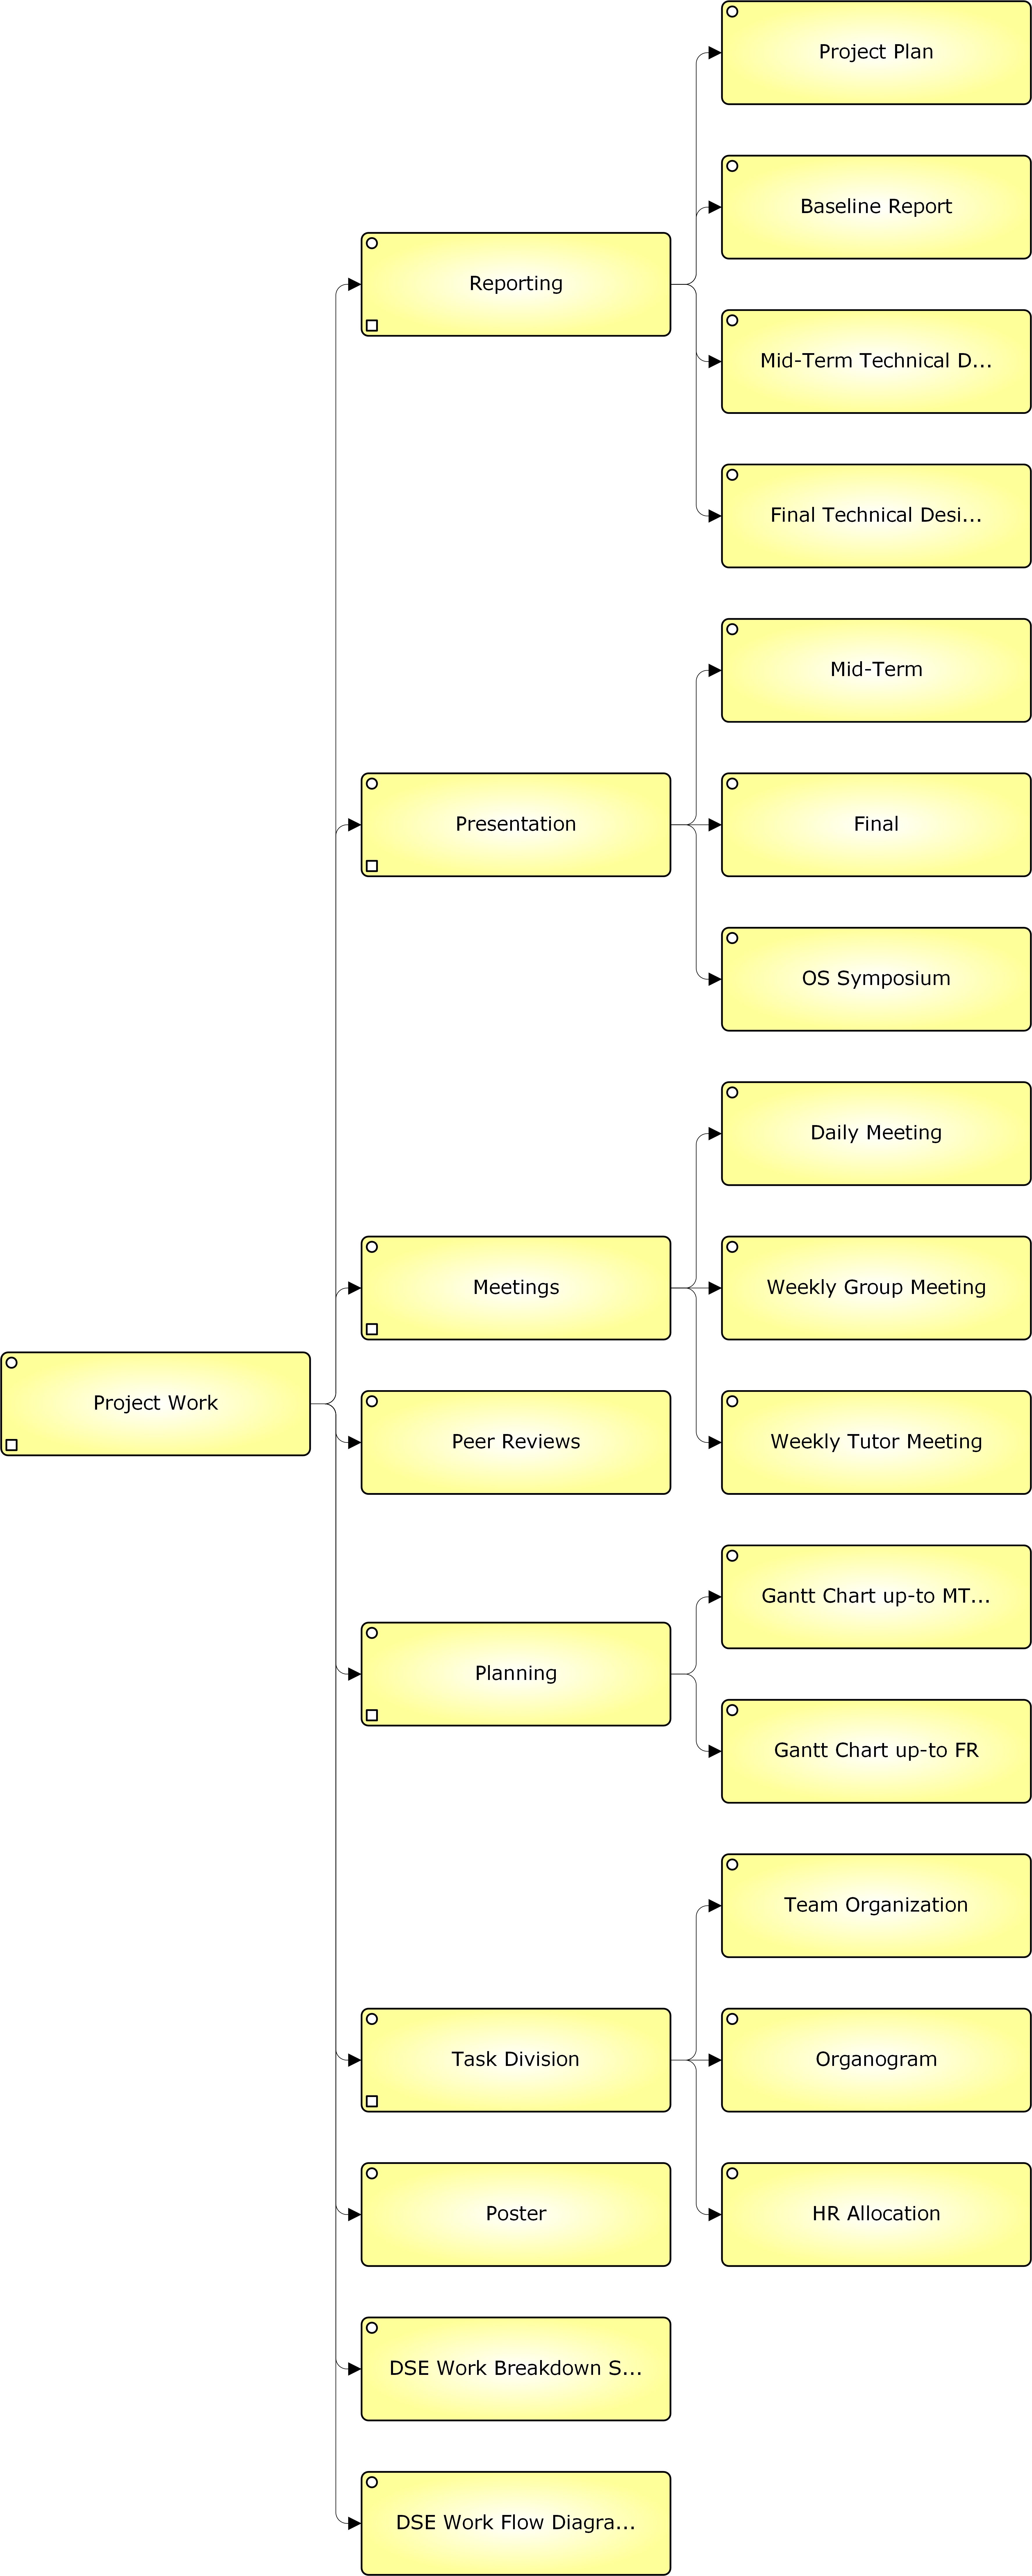
\includegraphics[height=20cm]{Figures/WBS_PW.png}

\caption{Project Work WBS tree}
\end{figure}



\end{document}
\end{appendices}
\end{document}